\documentclass[a4paper,12pt,oneside,openany]{book}
\usepackage{layout}
\setlength{\textwidth}{15.0 cm}
\setlength{\textheight}{25.0 cm}


\usepackage[english,brazil]{babel}
\usepackage{pagina} % pagina-padrao
\usepackage{indentfirst} % for indent
\usepackage[utf8]{inputenc}
\usepackage{graphics,epsfig}
\usepackage{graphics}
\graphicspath{{./figuras/}}
\usepackage{pstricks,pst-node,pst-tree}
\usepackage{alltt}
%\usepackage{makeidx}
%\makeindex
\usepackage[figuresright]{rotating} % for saydways tables and figures
\usepackage{enumerate} % for configuration of enumerate environment
\usepackage{amsmath}
\usepackage{amssymb}
\usepackage{portland,multirow}
\usepackage[chapter,ruled]{algorithm} % chapter for consistency with table and figures
\usepackage{algpseudocode}

\setcounter{secnumdepth}{3} % numeracao ate subsubsecao
\setcounter{tocdepth}{2} % indice ate subsubsecao

\usepackage{longtable}
\usepackage{hyperref}

\usepackage{nomes} % traduz pacotes suplementares ao babel

% cref command with adaptations to remove parentesis
\usepackage{cleveref}
\crefname{equation}{}{} % remove label
\crefformat{equation}{#2#1#3}
\crefrangeformat{equation}{#3#1#4-#5#2#6}
\crefmultiformat{equation}{#2#1#3}{ e~#2#1#3}{, #2#1#3}{ e~#2#1#3}


\begin{document}

\frontmatter
\thispagestyle{empty}


\includegraphics[scale=0.7]{Poli.eps}

\begin{center}
\large{PROCESSAMENTO DIGITAL DE IMAGENS E TEORIA DA COMPUTAÇÃO APLICADOS À MODELAGEM DOS PROCESSOS EMOCIONAIS HUMANOS}\\
   \vspace{2cm}
\large{Breno Vieira Arosa}\\
\end{center}
   \vspace{3cm}
\hspace{7cm}
\hfill \parbox{8.0cm}{Projeto de Graduação apresentado ao Curso de Engenharia Eletrônica e de Computação da Escola Politécnica, Universidade Federal do Rio de Janeiro, como parte dos requisitos necessários à obtenção do título de Engenheiro.\\}
   \vspace{2cm}
\hfill \parbox{8.0cm}{Orientador: Luiz Pereira Calôba} \\
   \vspace{2cm}
\begin{center}
Rio de Janeiro

Julho de 2017
\end{center}




\pagebreak


\begin{center}
\large{PROCESSAMENTO DIGITAL DE IMAGENS E TEORIA DA COMPUTAÇÃO APLICADOS À MODELAGEM DOS PROCESSOS EMOCIONAIS HUMANOS}\\
   \vspace{1cm}
\large{Breno Vieira Arosa}\\
\end{center}
   \vspace{2cm}
PROJETO DE GRADUAÇÃO SUBMETIDO AO CORPO DOCENTE DO CURSO DE ENGENHARIA ELETRÔNICA E DE COMPUTAÇÃO DA ESCOLA POLITÉCNICA DA UNIVERSIDADE FEDERAL DO RIO DE JANEIRO COMO PARTE DOS REQUISITOS NECESSÁRIOS PARA A OBTENÇÃO DO GRAU DE ENGENHEIRO ELETRÔNICO E DE COMPUTAÇÃO

   \vspace{1cm}
Autor:
      \vspace{0.5cm}
      \begin{flushright}
         \parbox{10cm}{
            \hrulefill

            \vspace{-.375cm}
            \centering{Breno Vieira Arosa}

            \vspace{0.1cm}
         }
      \end{flushright}


Orientador:
      \vspace{0.5cm}
      \begin{flushright}
         \parbox{10cm}{
            \hrulefill

            \vspace{-.375cm}
            \centering{Prof. Luiz Pereira Calôba, Dr. Ing.}

            \vspace{0.1cm}
         }
      \end{flushright}

Examinador:
      \vspace{0.5cm}
      \begin{flushright}
         \parbox{10cm}{
            \hrulefill

            \vspace{-.375cm}
            \centering{Prof Frances Elizabeth Allen, D. Sc.}

            \vspace{0.1cm}
         }
      \end{flushright}

Examinador:
      \vspace{0.5cm}
      \begin{flushright}
         \parbox{10cm}{
            \hrulefill

            \vspace{-.375cm}
            \centering{Prof. Alan Jay Perlis, D. E.}

            \vspace{0.1cm}
         }
      \end{flushright}


      \vfill


\begin{center}
Rio de Janeiro

Julho de 2017
\end{center}


\pagebreak

% Declaracao
\begin{center}
Declaração de Autoria e de Direitos
\end{center}

\vspace{0.5cm}

Eu, \emph{Breno Vieira Arosa} CPF \emph{131.187.117-95}, autor da monografia \emph{Aprendizado Semi-Supervisionado para Classificação de Polaridade de Tweets}, subscrevo para os devidos fins, as seguintes informações:\\
1. O autor declara que o trabalho apresentado na disciplina de Projeto de Graduação da Escola Politécnica da UFRJ é de sua autoria, sendo original em forma e conteúdo.\\
2. Excetuam-se do item 1. eventuais transcrições de texto, figuras, tabelas, conceitos e ideias, que identifiquem claramente a fonte original, explicitando as autorizações obtidas dos respectivos proprietários, quando necessárias.\\
3. O autor permite que a UFRJ, por um prazo indeterminado, efetue em qualquer mídia de divulgação, a publicação do trabalho acadêmico em sua totalidade, ou em parte. Essa autorização não envolve ônus de qualquer natureza à UFRJ, ou aos seus representantes.\\
4. O autor pode, excepcionalmente, encaminhar à Comissão de Projeto de Graduação, a não divulgação do material, por um prazo máximo de 01 (um) ano, improrrogável, a contar da data de defesa, desde que o pedido seja justificado, e solicitado antecipadamente, por escrito, à Congregação da Escola Politécnica.\\
5. O autor declara, ainda, ter a capacidade jurídica para a prática do presente ato, assim como ter conhecimento do teor da presente Declaração, estando ciente das sanções e punições legais, no que tange a cópia parcial, ou total, de obra intelectual, o que se configura como violação do direito autoral previsto no Código Penal Brasileiro no art.184 e art.299, bem como na Lei 9.610.\\
6. O autor é o único responsável pelo conteúdo apresentado nos trabalhos acadêmicos publicados, não cabendo à UFRJ, aos seus representantes,  ou ao(s) orientador(es), qualquer responsabilização/ indenização nesse sentido.\\
7. Por ser verdade, firmo a presente declaração.\\

      \vspace{0.5cm}
      \begin{flushright}
         \parbox{10cm}{
            \hrulefill

            \vspace{-.375cm}
            \centering{Breno Vieira Arosa}

            \vspace{0.1cm}
         }
      \end{flushright}

\pagebreak

% Copyright
\vspace{0.5cm}

UNIVERSIDADE FEDERAL DO RIO DE JANEIRO \\
Escola Politécnica - Departamento de Eletrônica e de Computação \\
Centro de Tecnologia, bloco H, sala H-217, Cidade Universitária \\
Rio de Janeiro - RJ      CEP 21949-900\\
\vspace{0.5cm}

Este exemplar é de propriedade da Universidade Federal do Rio de Janeiro, que poderá incluí-lo em base de dados, armazenar em computador, microfilmar ou adotar qualquer forma de arquivamento.

É permitida a menção, reprodução parcial ou integral e a transmissão entre bibliotecas deste trabalho, sem modificação de seu texto, em qualquer meio que esteja ou venha a ser fixado, para pesquisa acadêmica, comentários e citações, desde que sem finalidade comercial e que seja feita a referência bibliográfica completa.

Os conceitos expressos neste trabalho são de responsabilidade do(s) autor(es).

\pagebreak

% Dedicatória
\begin{center}
\textbf{DEDICATÓRIA}
\end{center}
\vspace{0.5cm}

\paragraph{}Opcional.

\pagebreak


% Agradecimento
\begin{center}
\textbf{AGRADECIMENTO}
\end{center}
\vspace{0.5cm}

\paragraph{}Sempre haverá. Se não estiver inspirado, aqui está uma sugestão: dedico este trabalho ao povo brasileiro que contribuiu de forma significativa à minha formação e estada nesta Universidade. Este projeto é uma pequena forma de retribuir o investimento e confiança em mim depositados.

\pagebreak

% Resumo
\begin{center}
\textbf{RESUMO}
\end{center}
\vspace{0.5cm}

As redes sociais modificaram a forma como as pessoas interagem e se tornaram cada vez mais presentes em suas vidas.
A produção de conteúdo digital, por sua vez, acompanha este crescimento.
Este grande volume de dados produzido dificulta o processo de extração de informações, uma vez que tais dados são
majoritariamente não estruturados.

O campo de processamento de linguagem natural nos dá ferramentas para de auxiliar a automatização desse procedimento.
Dentre estas técnicas, algoritmos de aprendizado de máquina se mostraram eficientes classificadores de texto em tarefas
como a análise de sentimento.
Em paralelo, observou-se nos últimos anos o aparecimento de técnicas de \textit{Deep Learning} que romperam barreiras
de desempenho nas mais diversas áreas da inteligência artificial.
Porém, a eficiência destes modelos depende de grandes bases de dados de treinamento, as quais têm processo de formação
custosas visto que a anotação destes dados é feita manualmente.

Este trabalho apresenta a elaboração de um método para gerar classificadores de \textit{Deep Learning} para análise de
sentimento de mensagens de redes sociais, sem a necessidade de bases de dados anotadas manualmente.
Para tal, serão formadas bases de dados com anotação ruidosa que servirão para treinamento de redes neurais
convolucionais.
Serão avaliados os resultados obtidos pelos classificadores de \textit{Deep Learning} em comparação com algoritmos de
aprendizado de máquina tradicionalmente aplicados no processamento de linguagem natural.

\vspace{1.0cm}

\noindent Palavras-Chave: Aprendizado de Máquina, Deep Learning, Processamento de Linguagem Natural, Análise de Sentimento.

\pagebreak

% Abstract
\begin{center}
\textbf{ABSTRACT}
\end{center}
\vspace{0.5cm}

Social networks have changed the way people interact and they become more and more present in their lives.
The production of digital content, in turn, accompanies this growth.
This large amount of data produced hinders the process of extracting information, since such data are mostly
unstructured.

Tools like natural language processing are able to aid automating this procedure.
Among these techniques, machine learning algorithms have been shown to be efficient text classifiers in tasks such as
sentiment analysis.
In parallel, it has been observed in recent years the emergence of Deep Learning techniques that have broken performance
barriers in the most diverse areas of artificial intelligence.
However, the efficiency of these models depends on large training datasets, which have a costly production process since
the labelling of this data is done manually.

This work presents the elaboration of a method for generating Deep Learning classifiers for sentiment analysis of social
networks messages without the necessity of manually annotated datasets.
In this respect, a dataset will be formed with noisy annotation and will be used to train convolutional neural networks.
The results obtained by the Deep Learning classifiers will be evaluated in comparison to machine learning algorithms
traditionally applied in natural language processing.

\vspace{1.0cm}

\noindent Keywords: Machine Learning, Deep Learning, Natural Language Processing, Sentiment Analysis.

\pagebreak

% Siglas
\begin{center}
\textbf{SIGLAS}
\end{center}
\vspace{0.5cm}

AdaGrad - Adaptative Gradient

Adam - \textit{adaptative moment estimation}

AUC - \textit{area under the curve}

CBOW - Continuos Bag-of-Words

CNN - redes neurais convolucionais

EMQ - Erro Médio Quadrático

GAN - redes neurais geradoras adversárias

LSTM - Long Short Term Memory

MLP - \textit{multilayer perceptron}

NB - Naïve Bayes

ReLU - \textit{rectified linear unit}

RNN - redes neurais recorrentees

ROC - \textit{receiver operating characteristic}

SemEval - \textit{Semantic Evaluation}

SVM - \textit{Suport Vector Machine}

TF-IDF - \textit{term frequence-inverse document frequence}

UFRJ - Universidade Federal do Rio de Janeiro

W2V - Word2Vec

\pagebreak


% Table of Contents
% ---------------------------------------------------------------
\tableofcontents
% ---------------------------------------------------------------
% Lista de figuras
% ---------------------------------------------------------------
%\cleardoublepage
%\addcontentsline{toc}{chapter}{Lista de Figuras}
\listoffigures
% ---------------------------------------------------------------
% Lista de Tabelas
% ---------------------------------------------------------------
%\cleardoublepage
%\addcontentsline{toc}{chapter}{Lista de Tabelas}
\listoftables
% ---------------------------------------------------------------
% Lista de Algoritmos
% ---------------------------------------------------------------
%\cleardoublepage
%\addcontentsline{toc}{chapter}{Lista de Algoritmos}
\listofalgorithms

\mainmatter
\cleardoublepage
% ---------------------------------------------------------------
% Chapter 1 - Introdução
% ---------------------------------------------------------------
\chapter{Introdução}
\label{introducao}
Neste capitulo serão descritos brevemente: o problema abordado, as áreas de conhecimento que cerceiam o estudo e os
métodos que compões a solução proposta por este trabalho.
Serão ainda ressaltados os motivos pelos quais o projeto apresentado é importante, assim como seus objetivos.

\section{Tema}

O tema do projeto é o estudo de técnicas de aprendizado de máquina para processamento de linguagem natural de redes
sociais.
Em especial, procura-se avaliar o impacto da utilização de técnicas de \textit{Deep Learning}, recentemente
desenvolvidas, quando aplicadas neste contexto.

O processamento de linguagem natural é o campo dentro de inteligência artificial que estuda a geração e compreensão de
línguas humanas.
Uma das principais características deste campo é o fato de ele lidar com dados não estruturados.
Nesse sentido, estudos que envolvam formas de comunicação, como por texto, apresentam diversas dificuldades.
Dentre elas estão: diferentes idiomas e alfabetos, variações linguísticas temporais e determinadas pelo meio em que a
mensagem está inserida, entre outros.
Soma-se a isso o fato de que apesar de estudos envolvendo o processamento de linguagem natural começarem a aparecer
desde a década de 50, as redes sociais são um fenômeno recente.
Por sua vez, estas se diferem de textos mais amplamente abordados principalmente por seu tamanho normalmente reduzido,
seu nível de formalidade e a frequente associação com mídias não textuais.
Tais distinções ressaltam a necessidade de desenvolvimento e validação de técnicas aplicadas especificamente ao contexto
de mídias sociais.

\section{Delimitação}

O objeto de estudo deste trabalho são os chamados \textit{tweets}, mensagens curtas publicadas na rede social Twitter.
O Twitter é uma das principais redes sociais, contando com 310 milhões de usuários ativos e gerando um total de meio
bilhão de \textit{tweets} por dia.

Sobre essas mensagens, será aplicada a análise de sentimento, cujo enfoque será a polaridade das mensagens,
separando-as entre positivas e negativas.
Não serão abordadas por esse projeto a objetividade ou neutralidade de um texto.

Por fim, o modelo a ser obtido visa à classificação de mensagens escritas em língua inglesa.
A língua inglesa foi escolhida por ter o maior conjunto de estudos e dados disponíveis.
Desta forma, é possível validar o método proposto comparando seus resultados com os obtidos na literatura.

\section{Justificativa}

As redes sociais são escolhidas como objeto de estudo por, ao longo da última década, ter se observado a massificação
de seu uso.
A medida que essas plataformas passam a ser cada vez mais relevantes, cresce a importância de se analisar o conteúdo
que trafega pelas redes.
Nesse meio de comunicação se encontram opiniões sobre assuntos, eventos ou produtos.
Neste quesito, é possível aplicar a análise de sentimento, ou mineração de opinião, que é o campo de estudo que visa a
resgatar as informações que transitam nos textos, de maneira a agregar conhecimento sobre os tópicos falados.

Entretanto, o crescimento da produção de dados inviabiliza o processo de análise manual deste conteúdo.
Logo, há a necessidade de técnicas, como a abordada por este trabalho, capazes de operar dados no volume em que são
gerados atualmente.

Em paralelo, observamos nos últimos anos o desenvolvimento do chamado \textit{Deep Learning}, que é uma família de
técnicas as quais tomam decisões em níveis mais altos de abstração.
Esses níveis são alcançados através do mapeamento obtido pelos dados através de redes neurais de diversas camadas.
Este conjunto de técnicas, viabilizadas pelo aumento de poder computacional apresentou sucesso nas mais diversas
aplicações, como no processamento de imagens, reconhecimento de fala, entre outros.
O campo do processamento de linguagem natural, por sua vez, foi fortemente impactado por estes algoritmos.
Ferramentas como redes neurais convolutivas, a princípio desenvolvidas para processamento de imagens e
\textit{Long Short-Term Memory}, propulsionaram o salto de desempenho obtido nos últimos anos.
O impacto deste avanço é notório no nosso dia a dia.
Frequentemente utilizamos, por exemplo, serviços automatizados de atendimento ao cliente ou ferramentas de tradução
simultânea que fazem uso desta abordagem.

É necessário ressaltar que parte do sucesso atribuído ao \textit{Deep Learning} provém de seu maior poder de abstração
dos dados.
Entretanto, essa característica faz com que haja uma dependência de grandes volumes de dados durante o treinamento
destes algoritmos.
Por esse motivo, ressalta-se a necessidade de métodos capaz de gerar bases de treinamento de maneira automática.

\section{Objetivos}

O objetivo deste projeto, portanto, consiste em formar um método de geração de modelos de \textit{Deep Learning} capazes
de sistematizar a classificação de sentimento de \textit{tweets}.
A produção destes modelos será feita de maneira a não depender de bases de dados anotadas manualmente, visto o alto
custo destas serem reproduzidas.

\section{Metodologia}

Para alcançar esse objetivo, o projeto foi dividido em três etapas: (1) replicar técnicas consolidadas de análise de
sentimento para \textit{tweets} sobre dados de treinamento obtidos por anotação automática; (2) formar uma base de dados
própria e aplicar os mesmos algoritmos utilizados anteriormente para validar o procedimento de sua elaboração; (3)
aplicar nos \textit{tweets} técnicas de \textit{Deep Learning} que vêm obtendo sucesso em processamento de linguagem
natural e avaliar o impacto das mesmas comparado-as a classificadores menos robustos.

A primeira etapa do trabalho será a replicação de estudos desenvolvidos por Go \textit{et al.}~\cite{go09}, que aplica
técnicas de \textit{Naïve Bayes} e \textit{Support Vector Machine} na classificação de polaridade de \textit{tweets},
sendo seu treinamento feito em cima de uma base de dados disponibilizada por Go \textit{et al.}, formada por anotação
automática.
Os resultados obtidos por estas técnicas serão utilizados como patamar para comparação dos modelos posteriormente
gerados.

Posteriormente, a segunda etapa consistirá em produzir uma base de treinamento gerada pelo método proposto por Go
\textit{et al.}, anotada automaticamente.
Para sua validação, serão replicados os mesmo algoritmos de \textit{Naïve Bayes} e \textit{Support Vector Machine},
os quais serão treinados com esse novo conjunto de dados e seus resultados são comparados aos obtidos pelos
classificadores do estágio anterior.

Finalmente, a terceira etapa fundamenta-se na aplicação de técnicas de \textit{Deep Learning}, como apresentadas por
Kim \cite{kim14}, em que se utiliza redes neurais convolucionais para classificação de texto.
O treinamento continua sendo feito a partir do banco de dados produzido por anotação automática, o qual foi apresentado
anteriormente.
Seus resultados serão comparados os obtidos pelos classificadores que compõem a etapa anterior, para analisar-se a
eficiência de algoritmos de \textit{Deep Learning} aplicados ao processamento de linguagem natural de redes sociais.

\section{Organização}

O Capítulo~\ref{contexto} aborda definições relevantes ao problema que será abordado.
Ele ressaltam-se a importância do objetivo proposto, situa o trabalho em sua área de conhecimento e apresenta o Twitter,
objeto do estudo.

O Capítulo~\ref{nlp} apresenta as técnicas necessárias para permitir o uso de aprendizado de máquina no processamento de
texto.
Este capítulo mostra as diferentes abordagens possíveis para transformações de texto em valores numéricos, ressaltando
como estas decisões afetam os algoritmos de aprendizado posteriormente aplicados.

Os algoritmos de aprendizado, por sua vez, são apresentados no Capítulo~\ref{supervisionado}.
Nele são explicitadas as fundamentações teóricas de cada algoritmo e variações necessárias para aplicações destas
técnicas em texto.
Também são apresentadas as métricas de avaliação de resultado que foram utilizadas para a realização do projeto.

O Capítulo~\ref{metodologia} descreve em detalhes cada etapa que compõe o trabalho.
Destaca-se os bancos de dados utilizados, a escolha dos parâmetros dos algoritmos de aprendizado e o procedimento
metodológico aplicado.

Já no Capítulo~\ref{resultados} são apresentados os resultados obtidos pelas técnicas de aprendizado de máquina propostas.
Neste Capítulo, os resultados encontrados são avaliados, comparados e discutidos.

Por fim, o Capítulo~\ref{conclusao} é composto pela conclusão, mostrando os objetivos cumpridos, destacando os ponto
positivos e apontando as limitações encontradas durante o desenvolvimento do projeto.
Nele são abordados também os possiveis trabalhos futuros.


% ---------------------------------------------------------------
% Chapter 2 - Posicionamento do Projeto
% ---------------------------------------------------------------
\chapter{Contextualização}
\label{contexto}
% Acertar titulo do capitulo

A internet apresenta um crescimento exponencial no mundo atual.
Estima-se que no ano de 2016 cerca de 66\% da população brasileira tenha acesso à rede \cite{social17}.
Ela é usada massivamente no dia a dia das pessoas, estando presente desde a realização de tarefas básicas e essenciais,
como cozinhar e se locomover numa cidade, até o preenchimento do tempo de lazer, com vídeos, notícias, mensagens
instantâneas e redes sociais.
% Falar sobre o uso da internet, ubuiquidade e etc

Através especialmente das redes sociais, a internet modificou a forma de interação entre as pessoas.
No Brasil, 58\% da população, ou seja, 120 milhões de pessoas, participam de pelo menos uma rede social, gastando em
média, 220 minutos por dia no ano de 2016~\cite{social17}.
Isso faz do Brasil o segundo país em tempo navegando em redes sociais, atrás apenas das Filipinas~\cite{social17}.
Essa situação não só cria uma nova instância de comunicação entre as pessoas, mas também abre um lugar para a expressão
dos sentimentos e opiniões de cada um.
Com isso, após o surgimento das redes sociais, a presença online por parte dos veículos de comunicação estabeleceu
um canal de via dupla.
Agora, os leitores interagem com a fonte de informação recebida, seja ela uma notícia, atualização de amigos, etc.

Essa presença central das mídias sociais na vida das pessoas faz com que os usuários passem a ser mais influenciados
por opiniões que trafegam pelas mesmas.
Desta maneira, as redes sociais passam a ter um peso maior na tomada de decisão de cada individuo, como na compra de
um produto ou na escolha de um candidato a ser votado.
Os impactos destes novos meios de comunicação podem ser observados, por exemplo, nas mobilizações de massa ocorridas na
primavera árabe em 2011, que levaram à queda de governos, tendo as mídias sociais exerceram papel
crítico~\cite{mourtada11} para tanto.

Nesse sentido, tornaram-se necessários trabalhos que analisem o que se está dizendo nas redes sociais.
Para uma emissora de TV, por exemplo, é interessante saber o que está sendo dito sobre sua programação, assim como para
a assessoria de um cantor é importante descobrir se sua nova canção está agradando ou não ao seu público.

Jim Yu, presidente da empresa de marketing digital BrightEdge, ressalta que os sentimentos expressos por clientes em
relação a uma marca é são uma das principais métricas de \textit{branding}~\cite{marketingland}.
Já o colunista da Forbes Daniel Newman destaca que a utilização de técnicas de análise de sentimento, em conjunto com
outras técnicas de \textit{big data}, vem revolucionando a forma de se fazer marketing, permitindo uma maior
personalização dos produtos e fortalecimento de relação com os clientes~\cite{newman16}.

Entretanto, a criação de conteúdo digital acompanha o crescimento da internet.
No ano de 2016, a cada sessenta segundos foram adicionadas 500 horas de vídeo no YouTube, realizadas 3.8 milhões de buscas
no Google e publicados 450 mil \textit{tweets}~\cite{smartinsights}.
Estes números tornam impraticável a realização de análise de sentimento manualmente sobre mídias com esse volume de
dados.
Portanto, a utilização de métodos automatizados é um modo de viabilizar a realização dessa tarefa.
Porém, a extração de informação de linguagem natural não é uma simples, pois envolve conhecimentos da língua explícitos
e implícitos, regulares e irregulares, sintáticos e semânticos~\cite{cambria13}.
Sobretudo, a análise de sentimento envolve problemas ainda não resolvidos no processamento de linguagem
natural~\cite{cambria13}, como a resolução de correferências~\cite{soon01}, resolução de anáforas~\cite{lappin94},
reconhecimento de entidades~\cite{nadeau07} e ambiguidade de palavras~\cite{yarowsky95}.
Estes fatores constituem desafios adicionais para a tarefa.

\section{Análise de Sentimento}

O campo de estudos da análise de sentimento, também chamado de mineração de opinião, é um dos ramos mais ativos do
processamento de linguagem natural~\cite{liu12}.
A análise de sentimento tem como objetivo analisar a opinião, a avaliação, a emoção e a atitude de um documento em
relação a um evento, produto, serviço, organização, ou qualquer outra entidade.
Apesar de o processamento de linguagem natural ter um longo histórico de estudos, a análise de sentimento se consolidou
apenas no inicio dos anos 2000 com a crescente demanda comercial.
Observa-se que o crescimento de interesse nessa área tem grande correlação com o crescimento de mídias sociais e do
volume de dados, visto que o sucesso das redes sociais disponibiliza quantidades massivas de dados, possibilitando tanto
a oferta de novas aplicações, quanto oportunidades de desenvolvimento de técnicas~\cite{liu12}.

O campo de análise de sentimento apresenta diferentes sub-áreas de estudo.
Dentre elas, a tarefa mais presente na literatura e que abordaremos neste trabalho é a análise de polaridade de um
documento.
A análise de polaridade visa a classificar textos em uma escala entre positivo e negativo.
Encontra-se também estudos que tem como objetivo determinar a subjetividade ou objetividade de um texto, como no
trabalho de Wiebe e Rilof~\cite{Wiebe05}.
Também entra no escopo de análise de sentimento a classificação de emoções presentes em uma mensagem, como felicidade,
raiva, tristeza, etc~\cite{bollen11b}.
Outro foco de pesquisa com grande aplicações práticas é a análise de sentimento porém, não da mensagem como um todo, mas
do sentimento em relação a uma entidade presente na mensagem~\cite{eirinaki12}.
O contrário também é possível, a análise da influência do sentimento de um termo em relação a mensagem~\cite{socher13}.
Percebe-se que a análise de sentimento se desmembra em varias subdivisões e novas subdivisões surgem a cada dia, visto
que a área ainda está em processo de expansão, o que confirma seu grande potencial de aplicação.

Com o crescimento da participação dos usuários na formação de conteúdo da Web, torna-se cada vez mais relevante a análise
do conteúdo sendo produzido.
Zhuang \textit{et al.}~\cite{zhuang06}, por exemplo, utiliza mineração de opinião para extrair avaliações a partir de
críticas de filmes feitas por usuários.
Hu e Liu~\cite{hu04}, por sua vez, desenvolveram métodos para resumo de sentimento de avaliações de produtos vendidos
por comercio eletrônico.

A utilização de classificadores de opinião sobre dados de redes sociais se mostrou relevante em diversas aplicações.
Bollen \textit{et al.}~\cite{bollen11}, por exemplo, aplicam análise de sentimento de mídias sociais para predição de
mercados financeiros.
Tumasjan \textit{et al.}~\cite{tumasjan10}, por sua vez, utilizam o sentimento exposto no Twitter para prever resultados
eleitorais.
Já Du \textit{et al.}~\cite{du14} empregaram análise de sentimento até mesmo na predição de bilheteria de filmes.

Porém, a produção de base de dados para o treinamento de modelos de aprendizado supervisionado é um processo custoso.
O seu processo de desenvolvimento envolve a anotação manual de dados, preferencialmente por múltiplas pessoas.
Contudo, apesar de modelos simples como os obtidos com técnicas como Naïve Bayes e \textit{Support Vector Machines}
conseguirem desempenhos satisfatórios com quantidades limitadas de dados, modelos mais complexos como redes neurais
profundas dependem de grandes volumes de dados para obter êxito, tornando o processo de anotação manual extremamente
ineficiente.
Sobretudo, uma vez formada esta base de dados, ela só é eficiente para o desenvolvimento de classificadores aplicados
na mesma língua, no mesmo formato, e sem grandes defasagens de tempo.
Por exemplo, uma base de dados composta por \textit{tweets} seria ineficiente para modelagem de classificadores de
emails, ou mesmo o uso de uma base formada por \textit{tweets} de 2010 sofreria queda de performance se o modelo
treinado com ela fosse aplicado em \textit{tweets} de 2018, visto a evolução da língua neste período de tempo.

Portanto, se faz necessário desenvolver métodos como o apresentado por Go \textit{et at.}~\cite{go09}, que desenvolve
uma base composta de \textit{tweets} a partir de anotação automática por \textit{emoticons}.
O trabalho de Go \textit{et at.}~\cite{go09} propõem-se a definir um sistema de classificação de sentimento sem a
necessidade de anotação manual dos dados para treinamento, utilizando supervisão distante, técnica de anotação ruidosa
automática.
Nesse artigo a análise de sentimento tratada é a extração de polaridade, negativa ou positiva, de uma mensagem.
Em especial, as mensagens desse trabalho são originárias do Twitter, serviço de microblogs, sendo esse trabalho o
primeiro a estudar este tipo de mensagem.

% colocar exemplos compativeis com os apresentados anteriormente
Por ser uma plataforma aberta, o Twitter é composto de mensagens dos mais diversos domínios.
Esse fator dificulta a tarefa de classificação a ser executada quando comparada a trabalhos de domínios específicos,
como por exemplo a análise de sentimento para avaliação de filmes a partir de resenhas; ou a predição de flutuações do
mercado financeiro pela análise de artigos jornalísticos.

A Tabela~\ref{tab:sentiment} exemplifica a classificação de polaridade de \textit{tweets}, foco deste trabalho.
As mensagens presentes nessa tabela são transcrições de \textit{tweets} reais, selecionados de maneira a ilustrar
a classificação de sentimento.

\begin{table}[h]
    \begin{center}
        \begin{tabular}{| l | p{10cm} |}
        \hline
        \textbf{Sentimento} & \textbf{\textit{Tweet}} \\ \hline
        Positivo & Grande notícia, João Sousa e Gastão Elias representam Portugal nos Jogos Olímpicos do Rio de Janeiro.
        \\ \hline
        Neutro & Entrevistei hoje a Priscilla Carnaval do BMX. Classificada para o \#Rio2016, ela tem novidades na
        preparação olímpica. \\ \hline
        Negativo & Estão transformando Olimpíadas que é algo sério num espetáculo triste e de mau gosto. \\ \hline
        \end{tabular}
        \caption{Exemplo de classificação de sentimento em \textit{tweets}.}
        \label{tab:sentiment}
    \end{center}
\end{table}

Entretanto, nem todos os exemplos são claramente distinguíveis como os apresentados na Tabela~\ref{tab:sentiment}.
A comunicação frequentemente apresenta fatores como ironia, ambiguidade de sentimentos e multiplicidade de idiomas.
Em outros casos, a mensagem sendo analisada pode ser complementar a mensagens anteriores ou informações não textuais
que a acompanham.
Esses fatores são complexidades adicionais e diminuem a acertividade dos classificadores.
A Tabela~\ref{tab:sentiment_complexity} demonstra exemplos das dificuldades indicadas.

\begin{table}[h]
    \begin{center}
        \begin{tabular}{| l | p{10cm} |}
        \hline
        \textbf{Fator} & \textbf{\textit{Tweet}} \\ \hline
        Ironia & Recomendo chegar para dar aula e descobrir que mudaram seu horário sem avisar. \\ \hline
        Ambiguidade & Estou igualmente fascinada e enojada. \\ \hline
        Multiplicidade de idiomas & Macarrão de arroz is the new miojo. \\ \hline
        \end{tabular}
        \caption{Dificuldades encontradas na classificação de sentimento.}
        \label{tab:sentiment_complexity}
    \end{center}
\end{table}

\section{Twitter}

O Twitter é um microblog e rede social no qual os usuários interagem a partir de mensagens, chamadas \textit{tweets}.
Microblogs são meios de comunicação que permitem aos usuários compartilhar conteúdos e mídias.
As principais características dos microblogs são a brevidade e instantaneidade.
Os \textit{tweets} são limitados a 140 caracteres e podem conter fotos, vídeos, links, localizações, referências a
usuários e \textit{hashtags}.
Criada em 2006, a rede social cresceu rapidamente a ponto de se tornar uma das redes com maior número de usuários no
mundo.
No ano de 2016, o Twitter contava com a presença de 330 milhões de usuários ativos por mês.
A Figura~\ref{fig:tweet_ex} mostra um exemplo de \textit{tweet}.

\begin{figure}
\begin{center} {
    \begin{center}
    
\includegraphics[scale=0.7]{tweet-example.png}
    \caption{Exemplo de \textit{tweet} contendo \textit{emoticon}, abreviação e neologismos.}
    \small{As informações do usuário foram anonimizadas para sua privacidade.}
    \label{fig:tweet_ex}
    \end{center}
}
\end{center}
\end{figure}

Um ponto chave da comunicação por Twitter são as \textit{hashtags}.
\textit{Hashtags} são palavras-chave ou frases que definem um tópico ou tema.
Elas são caracterizadas por serem precedidas pelo simbolo da tralha (\#) e por não conterem espaços ou pontuação.
São, ainda, elementos clicáveis que apontam o leitor para outra página.
Essa outra página, por sua vez, contém um mural com todas as citações contendo aquela \textit{hashtag}.
Desta forma, \textit{hashtags} funcionam como agregadores de \textit{tweets}.

O tamanho reduzido das mensagens veiculadas por Twitter e o meio pelo qual elas circulam levam à utilização de
variações gramaticais da língua especificas para este ambiente.
É comum encontrar, por exemplo, o uso excessivo de abreviações para reduzir a contagem total de caracteres, a repetição
de pontuação para reforçar intensidade e o uso de neologismos.

Se tratando de classificação de sentimento, o fato do tamanho reduzido e da linguagem própria apresentam uma dificuldade
adicional.
Apesar de não serem abordados nesse trabalho, atributos não textuais como republicação ou citação de mensagem, presença
de foto ou vídeo, grafos de conexões entre usuários etc. podem colaborar na realização da tarefa de análise de sentimento.


% ---------------------------------------------------------------
% Chapter 4 - NLP
% ---------------------------------------------------------------
\chapter{Processamento de Linguagem Natural}
\label{nlp}
O processamento de linguagem natural (NLP), é um dos principais ramos da Inteligência Artificial.
Um de seus marcos inicias desse área de conhecimento foi o teste de Turing~\cite{turing50} no qual propõe a capacidade
de comunicação como um critério de inteligência.
Desde sua criação, no inicio dos anos 50, o NLP se consolidou de maneira a se fazer presente no dia a dia das pessoas
como pode-se observar na utilização de serviços automatizados de atendimento ao clientes, ferramentas de tradução etc.
Grande parte destas aplicações provem da utilização de técnicas de aprendizado supervisionado como serão apresentados
no capitulo~\ref{supervisionado}.

As seções a seguir apresentam as transformações aplicadas a textos necessárias para viabilizar a aplicação de algoritmos
de aprendizado.

\section{Pré-processamentos}

A primeira etapa na preparação de uma mensagem para utilização em algoritmos de aprendizado de máquina é a separação por
palavras.
Este processo é chamado de \textit{tokenização}, denominando-se cada palavra resultante como token.
A \textit{tokenização} costuma incluir a separação de contrações como a transformação de \textit{dela} em \textit{de}
e \textit{ela}.

% figura mostrando tokenização

Para aplicação de tarefas como a de classificação é comum se remover as palavras mais comuns de um idioma e que não
agregam informação discriminantes para o objetivo desejado, essas palavras são chamadas de \textit{stopwords}.
A remoção de \textit{stopwords} visa reduzir o ruído presente em dados textuais, aumentando a acurácia dos algoritmos de
aprendizado de máquina e reduzindo a complexidade do problema~\cite{silva03}.
Porém, a remoção de \textit{stopwords} provindas de listas pré compiladas, técnica mais utilizada, apresenta desafios
principalmente devido a dinamicidade de meios como redes sociais.
Saif \textit{et al.}~\cite{saif14} apresentam um estudo comparativo do efeito da remoção de \textit{stopwords} por
diferentes técnicas e seus efeitos na classificação de sentimento de \textit{tweets}.
Além da remoção de \textit{stopwords}, em mensagens provindas de redes sociais também são costumeiramente removidos
links, \textit{hashtags} e menções a usuários.

Também é possível realizar a correção ortográfica das palavras e a lematização, processo de extração do radical da
palavra.
Estas técnicas são normalmente empregadas para reduzir o vocabulário e diminuir assim a complexidade do treinamento.

\section{Representações Numéricas}

Contudo, a utilização de algoritmos de aprendizado de máquina depende de uma representação numérica dos dados.
Portanto, após a conversão de uma mensagem em uma uma sequência de tokens, há uma etapa de transformação destas cadeias
de tokens em matrizes ou vetores.
Serão apresentadas nas subseções seguintes as principais técnicas referentes a este processo.

\subsection{Codificação One-Hot}

Um dos métodos mais observados na literatura é a codificação \textit{one-hot}, na qual cada token é representado de
maneira maximamente esparsa.
Ou seja, é definido um espaço cujo número de dimensão é dada pelo tamanho do vocabulário utilizado e cada palavra é
substituída por um vetor unitário na direção que representa sua posição no vocabulário.
Desta maneira, cada token é representado por um vetor unitário de dimensão igual a do vocabulário.

Outra forma possível de utilização é transformar cada par de palavras em um token.
A utilização de múltiplas palavras por token é chamada de \textit{n-gram}.
A ideia da aplicação de \textit{n-gram} é capturar expressões ou distinguir palavras em diferentes contextos.
Porém, sua utilização aumenta significativamente o tamanho do vocabulário, podendo dificultar o processo de treinamento.

\subsection{Bag-of-Words}

Uma vez que cada palavra é caracterizada por sua codificação \textit{one-hot}, a forma natural de simbolizar uma mensagem
é por uma matriz na qual cada coluna é composta pelo vetor correspondente a cada palavra da frase.
Contudo, para evitar o aumento da dimensionalidade do problema é comum se utilizar da técnica \textit{bag-of-words} na
qual cada mensagem é representada pela soma dos vetores de seus tokens~\cite{schutze08}.

Esta técnica também é chamada na literatura como \textit{term frequence} (tf), dado que a técnica é dada pela contagem
de termos de um documento.
Nesse caso as palavras são pesadas igualmente, outra abordagem possível é multiplicar a frequência do termo no documento
pelo inverso do número de documentos no qual aquele termo aparece, técnica denominada \textit{term frequence-inverse
document frequence} (TF-IDF)~\cite{salton88}.
A TF-IDF permite compensar a grande presença de palavras muito frequentes, que limitariam a influência de termos pouco
usados.

É possível notar que a utilização de ambas as técnicas ignora a ordem das palavras na frase.
Técnicas como Word2Vec, apresentada na seção~\ref{sec:w2v}, permitem a utilização da posição do termo na mensagem por conter
uma representação densa de cada token, reduzindo a dimensionalidade do problema.

\subsection{Word2Vec} \label{sec:w2v}

Word2Vec~\cite{mikolov13} (W2V) é uma técnica que visa representar uma palavra por um vetor de números reais, denso e de
tamanho arbitrário.
Os resultados obtidos por Mikolov \textit{et at.}~\cite{mikolov13} mostram que a representação vetorial é capaz de
capturar parte do sentido semântico dos termos.
Na prática, isso significa que, por exemplo, palavras sinônimas ficam próximas entre si no \textit{embedding} obtido.

Desenvolvida por um grupo de engenheiros do Google, estes vetores são aprendidos a partir de uma janela de contexto
ao redor de cada palavra presente nos documentos de treinamento.

Foram desenvolvidos dois modelos de treinamento distintos, são eles o \textit{Continuos Bag-of-Words} (CBOW) e o
\textit{Skipgram}.
A diferença entre ambos, além da forma de treinamento, se dá principalmente pelo tempo de convergência e pela acurácia.
No treinamento por CBOW, o W2V visa prever o termo central da janela a partir das palavras que a rodeiam.
No modelo obtido por \textit{Skipgram} o treinamento, por sua vez, é dado de forma a prever as palavras de contexto a
partir do termo central da janela.

O modelo Word2Vec se constitui de uma rede neural de uma única camada escondida em que suas entradas e objetivos são a
codificação \textit{one-hot} dos termos.

O número de neurônios presentes na camada escondida equivale a dimensionalidade do \textit{embedding}.
No caso do treinamento por CBOW a entrada é da rede é dada por palavras de contexto, ou seja, as palavras ao redor do
termo a ser treinado, sendo esse termo o objetivo da rede.
A sua primeira camada possui ativação linear, com coeficiente $\frac{1}{c}$ no qual $c$ representa o tamanho da janela
utilizada.
Enquanto a segunda camada é composta por ativação \textit{softmax}.
O treinamento do modelo \textit{Skipgram} é análogo, porém com as entradas e saídas invertidas.
Os pesos do modelo Word2Vec são os obtidos na primeira camada após o treinamento da rede.

Por não necessitar de anotação se faz possível a utilização de conjuntos massivos de textos no treinamento do Word2Vec.
Entretanto, apesar do uso de grandes volumes de dados permitir um melhor desempenho do modelo esse fator também aumenta
significativamente o tempo de treinamento.
Para abordar esse problema, Mikolov \textit{et al.}~\cite{mikolov13b} apresentam uma técnica de treinamento com
amostragem, acelerando o processo significativamente.

Apesar de ser o \textit{embedding} mais conhecido para representação de texto, outros grupos de pesquisadores
desenvolveram técnicas com a mesma finalidade.
Dentre elas, destacam-se GloVe~\cite{pennington14}, algoritmo desenvolvido por um grupo de pesquisadores de Stanford e
FastText~\cite{bojanowski16}, produzido por uma equipe do Facebook.


% ---------------------------------------------------------------
% Chapter 3 - Aprendizado Supervisionado
% ---------------------------------------------------------------
\chapter{Aprendizado Supervisionado}
\label{supervisionado}
O aprendizado supervisionado é o campo dentro de aprendizado de máquina que visa a gerar modelos preditores a partir de um conjunto de dados de treinamento cujos resultados são previamente conhecidos.

\section{Naive Bayes}

\textit{Naive Bayes} é uma das técnicas mais simples disponíveis nesse contexto. Ela se baseia no teorema de Bayes enquanto assume independência entre as características escolhidas para descrever o dado. Abaixo veremos sua formulação matemática como descrita por Schütze \cite{schutze08}.

Tendo $\mathbf{x}$ tal que $\mathbf{x} \in \mathbf{X}$ em que $\mathbf{X}$ é o conjunto de dados de treinamento, a sua probabilidade de pertencer a classe $c_k \in \mathbf{c}$ é dada pelo teorema de Bayes:
\begin{equation} \label{eq:bayes}
    p(c_k \mid \mathbf{x}) = \frac{p(c_k) \ p(\mathbf{x} \mid c_k)}{p(\mathbf{x})}
\end{equation}

Sendo $\mathbf{x}$ um vetor de $n$ características, ao se assumir independência entre elas obtém-se:
\begin{equation}
    p(x_i \mid x_{i+1}, \dots ,x_{n}, c_k ) = p(x_i \mid c_k)
\end{equation}

Logo, pode-se rescrever a equação \ref{eq:bayes} substituindo $p(\mathbf{x} \mid c_k)$ pelo produtório de suas características:
\begin{equation}
    p(c_k \mid \mathbf{x}) = \frac{p(c_k) \prod_{i=1}^n p(x_i \mid c_k)}{p(\mathbf{x})}
\end{equation}

Como $p(\mathbf{x})$ será uma constante dado cada exemplo $\mathbf{x}$ esta pode ser desprezada:
\begin{equation}
    p(c_k \mid \mathbf{x}) \propto p(c_k) \prod_{i=1}^n p(x_i \mid c_k)
\end{equation}

Portanto, tem-se que o estimador ótimo $\hat{y}$ escolherá pela classe que atinja maior probabilidade:
\begin{equation}
    \hat{y} = \underset{k \in \{1, \dots, K\}}{\operatorname{max}} \ p(c_k) \displaystyle\prod_{i=1}^n p(x_i \mid c_k)
\end{equation}

Vê-se então que o modelo de \textit{Naive Bayes} depende apenas de $p(c_k)$ e $p(\mathbf{x} \mid c_k)$. Estes parâmetros serão extraídos do conjunto de treino por máxima verosimilhança.

Dado um vetor $\mathbf{y}$ de tamanho $m$ que representa as classificações referentes a $\mathbf{X}$, pode-se estimar $p(c_k)$ pela contagem de vezes que a classe $c_k$ aparece no conjunto de treinamento:
\begin{equation}
    \hat{p}(c_k) = \frac{\sum_{i=1}^m [y_i = c_k]}{m}
\end{equation}

Por sua vez, $p(x_r \mid c_k)$ é estimado utilizando a contagem de vezes que uma característica aparece dividida pelo total de características presentes em $\mathbf{X'}$ que é o subconjunto de treino pertencente a classe $c_k$:
\begin{equation}
    \hat{p}(x_r \mid c_k) = \frac{\sum_{j=i}^{m'} \sum_{i=1}^n [x_{ji} = x_r]}{|\mathbf{X'}|}
\end{equation}

Vê-se que modelos montados a partir de \textit{Naive Bayes} são computacionalmente baratos dado que seus parâmetros são obtidos através de contagens sobre os dados de treinamento e que sua predição utiliza apenas multiplicações.
Embora se baseie na independência entre características, seu baixo custo operacional leva esta técnica a ser utilizada mesmo em problemas com notória dependência de características como a classificação de texto \cite{mccallum98}.

\section{SVM}

O conceito fundamental do \textit{Support Vector Machine} se dá pela obtenção de um vetor de suporte que melhor separe as classes. Esta separação é feita de maneira que se maximize a margem entre as classes. A figura \ref{fig:svm} demostra dados de duas classes distintas, representadas pelas cores rosa e amarelo, pertencentes a um espaço de características de duas dimensões; vê-se na figura que a reta que define a maior separação é suportada pelos dados de cada classe mais próximos a ela.

\begin{figure}
\begin{center} {
    \begin{center}
    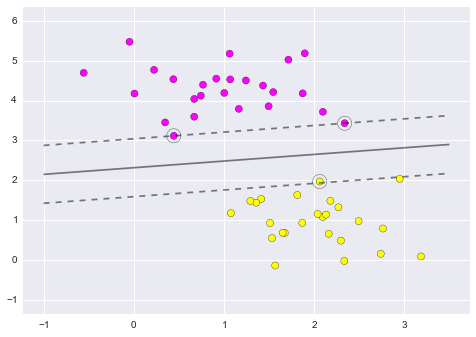
\includegraphics[scale=0.7]{svm.png}
    \caption{Reta de maior margem entre classes.}
    \small Imagem com direitos cedidos para uso não comercial, retirada de \cite{vanderplas15}
    \label{fig:svm}
    \end{center}
}
\end{center}
\end{figure}

Por se basear nos dados próximos ao limiar de separação das classes, o algoritmo passa a ser incapaz de distinguir os casos de classes que não são separáveis sem erros. A solução desse problema foi a criação de uma variável de relaxamento que define um número máximo de erros de classificação permitido. Esta propriedade é descrita com mais detalhes por Cortes e Vapnik em \cite{cortes95}. Sua utilização permite o desenvolvimento de modelos mais robustos a \textit{outliers} e melhora a generalização. Outros exemplos de regularizadores, como este, serão apresentados na subseção \ref{sec:regularizadores}.

Como utilizam vetores de suporte para definir hiperplanos de separação, SVMs não são capazes de segregar classes não linearmente distinguíveis. Podemos observar um exemplo deste caso na figura \ref{fig:svm-lin}, na qual um SVM treinado tenta separar classes concêntricas.

\begin{figure}
\begin{center} {
    \begin{center}
    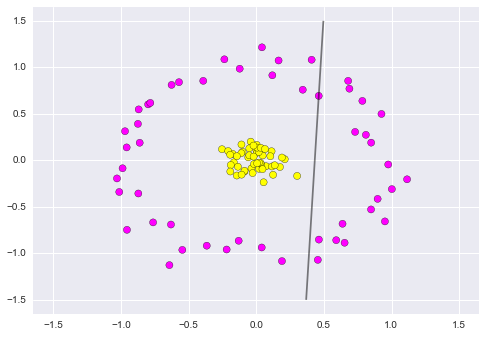
\includegraphics[scale=0.7]{svm-lin.png}
    \caption{SVM em dados não linearmente separáveis.}
    \small Imagem com direitos cedidos para uso não comercial, retirada de \cite{vanderplas15}
    \label{fig:svm-lin}
    \end{center}
}
\end{center}
\end{figure}

Para contornar esse impedimento, foi elaborado o que se chamou de \textit{kernel trick}. Este se baseia em um mapeamento não linear dos dados para um espaço onde possam ser linearmente separáveis \cite{scholkopf02}. A figura \ref{fig:svm-rbf} mostra a representação dos dados apresentados na figura \ref{fig:svm-lin} após seu mapeamento por uma função de base radial.

\begin{figure}
\begin{center} {
    \begin{center}
    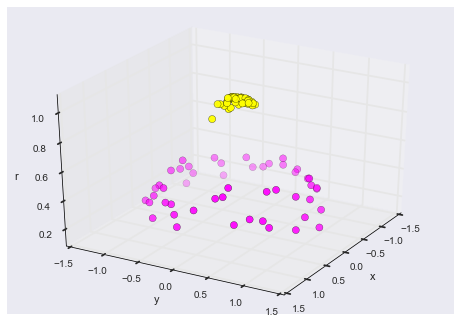
\includegraphics[scale=0.7]{svm-rbf.png}
    \caption{Transformação de dados por função de base radial.}
    \small Imagem com direitos cedidos para uso não comercial, retirada de \cite{vanderplas15}
    \label{fig:svm-rbf}
    \end{center}
}
\end{center}
\end{figure}

Neste novo espaço definido pela transformação, os dados são linearmente separáveis. Portanto, é possível achar um vetor de suporte que defina um hiperplano de separação das classes. Vemos na figura \ref{fig:svm-rbf-clas} as margens encontradas.

\begin{figure}
\begin{center} {
    \begin{center}
    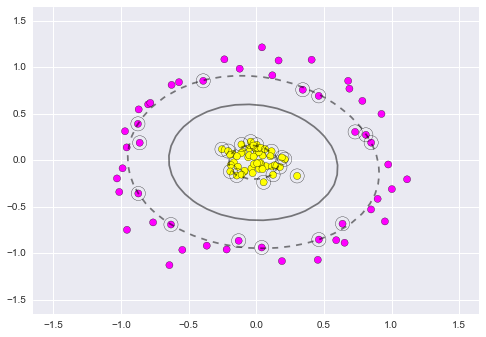
\includegraphics[scale=0.7]{svm-rbf-clas.png}
    \caption{SVM com \textit{kernel} de base radial.}
    \small Imagem com direitos cedidos para uso não comercial, retirada de \cite{vanderplas15}
    \label{fig:svm-rbf-clas}
    \end{center}
}
\end{center}
\end{figure}

Uma limitação na utilização deste algoritmo é seu tempo de treinamento. Sua complexidade computacional fica entre $O(n_{caracteristicas} \times n_{dados}^2)$ e $O(n_{caracteristicas} \times n_{dados}^3)$ \cite{list09}. Porém, Suykens e Vandewalle desenvolveram uma função custo através da qual tornou possível realizar o treinamento de SVMs a partir da otimização pelo método do gradiente \cite{suykens99}.

\section{Redes Neurais}

Redes Neurais são sistemas computacionais que visam replicar o modelo de processamento do cérebro. Há diversas variações de Redes Neurais. Nesta subseção será abordada a mais simples, Redes Neurais FeedForward, e na subseção \ref{sec:convolucionais} serão apresentadas Redes Neurais Convolucionais.

Redes Neurais FeedForward são compostas de camadas de neurônios sucessivamente interligadas por sinapses. As sinapses funcionam como um ponderador linear dos neurônios da camada anterior. Os neurônios, por sua vez, representam uma função de ativação, normalmente não linear, tais como: tangente hiperbólica, logística etc. Como exemplificação, há a figura \ref{fig:ff-neural-net}, onde apresenta-se o diagrama de uma rede que conta com uma camada de entrada que representa os dados do problema, seguida de duas camadas intermediarias, comumente chamadas de escondidas, as quais são seguidas pela camada de saída, que apontará o resultado final de todo processamento da rede.

\begin{figure}
\begin{center} {
    \begin{center}
    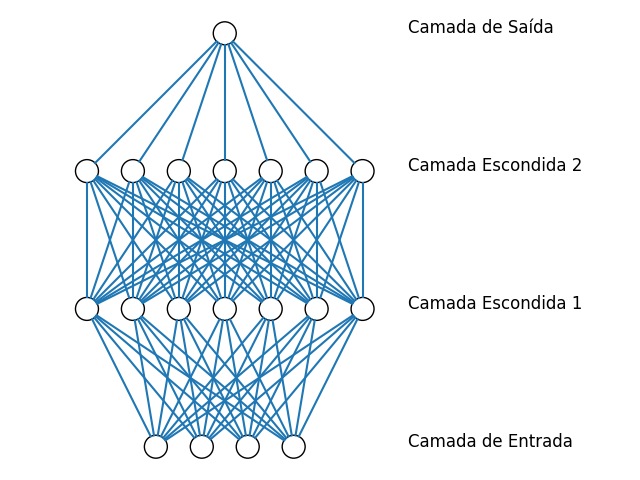
\includegraphics[scale=0.75]{ffnn.png}
    \caption{Rede Neural FeedFoward}
    \label{fig:ff-neural-net}
    \end{center}
}
\end{center}
\end{figure}

Uma de suas principais características de Redes Neurais é a capacidade de aproximar qualquer função, dado que a rede contenha pelo menos uma camada escondida com número suficientemente grande de neurônios com ativação não linear \cite{hornik89}.

Para uma Rede Neural simular uma função, precisa-se obter o conjunto de pesos, ou sinapses, que torne esta rede uma boa representação para a função escolhida. Em outras palavras, precisa-se minimizar o erro da representação da rede dado que este erro é uma função das sinapses. Uma prática comum é inicializar a rede com pesos selecionados de uma distribuição uniforme com média zero e desvio padrão inversamente proporcional ao número de dados de treinamento \cite{lecun12}. Posteriormente, é feita uma otimização da representação em função dos pesos. Para realizar esta otimização, utiliza-se normalmente \textit{Backpropagation} para se encontrar o ajuste ideal de cada sinapse baseada, em sua contribuição no erro. Uma explicação deste método é apresentada por Williams e Hinton em \cite{williams86}.

\subsection{Deep Learning}

O sucesso na aplicação de Redes Neurais nas mais diversas áreas levou à utilização de redes cada vez mais robustas. Assim, Redes Neurais profundas romperam barreiras de performance em problemas como reconhecimento de fala, detecção de objetos, tradução etc \cite{lecun15}. Chamou-se de \textit{Deep Learning} o campo de estudo de Redes Neurais com muitas camadas.

Cada camada de uma Rede Neural gera uma abstração que representa a sua entrada de modo a facilitar a tarefa a ser realizada. O encadeamento de camadas resulta em representações mais complexas dos dados, revelando relações previamente não observáveis. O aprofundamento das redes visa a reduzir ou eliminar a chamada \textit{feature engineering}, processo de seleção de características, que usualmente requer expertise no domínio do problema. Considerando por exemplo o caso do diagnóstico de câncer de pele, técnicas tradicionais de classificação dependiam de extração de informações de imagens de lesões, tais como: formato, tamanho, cor etc. Modelos baseados em Redes Neurais profundas são capaz de obter resultados superiores, eliminando completamente esta etapa \cite{esteva17}.

\subsection{Redes Neurais Convolucionais} \label{sec:convolucionais}

A utilização de Redes Neurais FeedForward em imagens sofre limitações, por cada pixel estar diretamente ligado aos neurônios, rotações ou translações na imagem afetam fortemente a capacidade da rede. Pretendendo solucionar estes problemas, foram desenvolvidadas Redes Neurais Convolucionais, cujas conexões são baseadas no funcionamento do córtex visual.

Elas são compostas primariamente de dois tipos de camadas: convolucionais e \textit{pooling}. Camadas convolucionais são formadas por um conjunto de filtros espaciais compostos das mesmas funções não-lineares utilizadas em Redes Feedforward \cite{goodfellow16}. Para cada exemplo do conjunto de dados, o filtro, cujo tamanho é menor que a entrada, é aplicado no inicio do dado e deslocado até o final. Desta forma, os filtros dividem os pesos entre todo espaço do dado, permitindo uma insensibilidade a deslocamentos e rotações. Por sua vez, as camadas de \textit{pooling} visam reduzir o número total de sinapses da rede. Para tal, reduz-se o tamanho dos filtros, obtendo-se valores máximos ou médias de dimensões desses filtros. \textit{Pooling} é fundamental quando o objetivo a ser atingido depende mais da presença de uma característica do que sua sua posição no dado \cite{goodfellow16}.

Por fim, apesar de Redes Convolucionais terem sido desenvolvidas com intuito de solucionar problemas de visão computacional, elas também obtiveram êxito nas mais diversas áreas, como no reconhecimento de voz e em séries temporais \cite{lecun95}. Tal sucesso pode ser atribuído à insensibilidade da rede a deslocamentos.

\section{Otimizadores}
% deep learning book

\subsection{SGD}

\subsection{Momentum}

\subsection{RMSProp}

\subsection{Adam}

\section{Regularizadores} \label{sec:regularizadores}
% overfit

\subsection{L2}

\subsection{Dropout}

\section{Supervisão Distante}


% ---------------------------------------------------------------
% Chapter 5 - Metodologia
% ---------------------------------------------------------------
\chapter{Metodologia}
\label{metodologia}
Este capítulo tem como objetivo descrever a elaboração de modelos de aprendizado de máquina capazes de classificar
sentimento, positivo ou negativo, de \textit{tweets}.
A produção desse modelo será feita a partir de base de dados anotada de maneira automatizada, permitindo a sua
fácil replicação.

\section{Bases de Dados} \label{sec:data}

O trabalho Sentiment140, desenvolvido por Go \textit{et al.}~\cite{go09} visa a definir um sistema de classificação de
sentimento sem a necessidade de anotação manual dos dados para treinamento, utilizando a técnica de supervisão distante.
Conjuntamente com o artigo, Go \textit{et al.} disponibilizaram um base de dados formada por supervisão distante composta
de 800 mil \textit{tweets}, divididos igualmente entre as classes positivas e negativas, e uma pequena base de testes de
360 \textit{tweets} anotados manualmente, também divididos igualmente entre as classes.

A não dependência de anotação dos dados e a facilidade de coleta dos \textit{tweets}, por meio de interface programável,
viabilizam a formação de uma grande base de treinamento.
Para a realização deste trabalho foram coletados cerca de 40 milhões de mensagens amostradas do conjunto total de
\textit{tweets}, filtrando-as apenas pelo idioma inglês.
Essas mensagens foram coletadas entre os anos de 2015 e 2017 a partir de interface programável oferecida pelo Twitter.

Posteriormente, se aplicou o método de classificação ruidosa de sentimento desenvolvido por Read~\cite{read05} como
especificado na Seção~\ref{sec:distant_supervision} nos \textit{tweets} coletados.
Nesse método, são definidos grupos de \textit{emoticons} positivos e negativos.
Mensagens que possuíram \textit{emoticons} pertencentes a algum destes grupos foram anotadas com as respectivas classes.
Caso \textit{emoticons} de ambos os grupos estejam presentes em uma mesma mensagem esta será descartada.
Os \textit{emoticons} utilizados para anotação da base de dados foram removidos das mensagens para evitar introduzir
viés ao classificador.

A Tabela~\ref{tab:emoticons} mostra os \textit{emoticons} escolhidos para compor a anotação ruidosa.
Em adição aos \textit{emoticons} presentes no Sentiment140, foram classificados manualmente os emoticons com maior
número de aparições nas mensagens coletadas.
Estudos indicam que a escolha dos \textit{emoticons} pode definir quão ruidosa é a anotação automática.
Durante este processo, observou-se um grande desbalanceamento entre classes, na qual os \textit{tweets} positivos
compõem 80\% do volume total de anotações.

\begin{table}[h]
    \begin{center}
        \begin{tabular}{| c | c |}
        \hline
        \textbf{Negativos} & \textbf{Positivos} \\ \hline
        :( & :) \\ \hline
        =( & =) \\ \hline
        :-( & :-) \\ \hline
        :'( & :D \\ \hline
        
\includegraphics[height=1em]{emojis/1F62D.pdf} & 
\includegraphics[height=1em]{emojis/1F60D.pdf} \\ \hline
        
\includegraphics[height=1em]{emojis/1F612.pdf} & 
\includegraphics[height=1em]{emojis/1F602.pdf} \\ \hline
        
\includegraphics[height=1em]{emojis/1F622.pdf} & 
\includegraphics[height=1em]{emojis/1F60D.pdf} \\ \hline
        
\includegraphics[height=1em]{emojis/1F614.pdf} & 
\includegraphics[height=1em]{emojis/1F60A.pdf} \\ \hline
        
\includegraphics[height=1em]{emojis/1F62A.pdf} & 
\includegraphics[height=1em]{emojis/1F618.pdf} \\ \hline
                                                       & 
\includegraphics[height=1em]{emojis/1F495.pdf} \\ \cline{2-2}
                                                       & 
\includegraphics[height=1em]{emojis/2665.pdf} \\ \cline{2-2}
                                                       & 
\includegraphics[height=1em]{emojis/2764.pdf} \\ \cline{2-2}
                                                       & 
\includegraphics[height=1em]{emojis/1F49B.pdf} \\ \cline{2-2}
                                                       & 
\includegraphics[height=1em]{emojis/1F499.pdf} \\ \cline{2-2}
                                                       & 
\includegraphics[height=1em]{emojis/1F49A.pdf} \\ \hline


        \end{tabular}
        \caption{Emoticons selecionados para aplicação de supervisão distante.}
        \label{tab:emoticons}
    \end{center}
\end{table}

A base de teste, por sua vez, é composta de \textit{tweets} anotados manualmente.
Essa base é formada pela coletânea de dados disponibilizados pela conferencia anual \textit{Semantic Evaluation}
(SemEval)~\cite{semeval17} entre os anos 2013 e 2017.
Esta base é composta de cerca de 70 mil \textit{tweets} e classificados entre positivos, neutros ou negativos.
Como este trabalho considera apenas as classes positivas e negativas, foram descartados as mensagens neutras.
O processo de anotação destes dados foi feito manualmente através da plataforma CrowdFlower, na qual cada mensagem
foi avaliado por pelo menos 5 pessoas e a anotação foi considerada válida se 3 ou mais participantes apresentaram a
mesma avaliação, como descrito por Rosenthal \textit{et al.}~\cite{rosenthal17}, organizadores do evento.
Novamente foram removidos os \textit{emoticons} presentes na anotação ruidosa para evitar introdução de tendência.

\section{Figuras de Mérito} \label{sec:metrics}

Uma vez definidos os dados, se faz necessário definir como será avaliada a performance dos modelos a serem treinados.
Esta seção apresentará as figuras de mérito utilizadas para seleção de parâmetros e avaliação dos algoritmos.

A forma mais direta de se medir a performance de um modelo é considerar a sua acurácia, que é a média aritmética das
eficiências de cada uma das classes.
Todavia, a presença de desbalanceamento de classes nos dados pode favorecer a acertividade da classe mais presente
enquanto perde eficiência na classificação da classe com menos exemplos.

% ROC - dissertacao fernando
A curva ROC (\textit{receiver operating characteristic})~\cite{bradley97} é uma forma de visualizar a performance de um
classificador binário para seleção de um ponto de operação.
Nela, a probabilidade de detecção e falso alarme variam com a escolha do patamar de decisão.
Um classificador ideal, que atinge 100\% de probabilidade de detecção sem nenhum caso de falso alarme, é representado na
curva ROC como um degrau.
Desta forma, a área sob a curva (AUC) pode ser utilizada como valor numérico de eficiência para um classificador.

% SP - dissertacao fernando
O índice SP~\cite{ciodaro12} é outro método de avaliação de classificadores binários.
A Equação~\ref{eq:sp} descreve a formação desse índice na qual $P_c$ representa a probabilidade de detecção da classe
positiva enquanto $P_{nc}$ caracteriza a probabilidade de não obtenção de falso alarme.

\begin{equation} \label{eq:sp}
    SP = \sqrt{\sqrt{P_c P_{nc}} \left(\frac{P_c + P_{nc}}{2}\right)}
\end{equation}

O patamar de decisão do classificador treinado será escolhido de maneira a maximizar o índice SP.
Pois este será um ponto de operação que apresenta um compromisso entre a eficiência de ambas as classes.

% validaçao cruzada, ver dissertação do junior
Uma maneira de garantir que os resultados obtidos pelas figuras de mérito apresentadas sejam consistentes independente do
conjunto de dados na qual será aplicado é utilizar a validação cruzada.
Neste trabalho será utilizado o método de validação cruzada de K-partições~\cite{kohavi95}.
Este processo consiste na separação aleatória da base de dados em $k$ conjuntos mutualmente exclusivos de tamanhos
similares.
Posteriormente são executadas $k$ rodadas, na qual o conjunto correspondente a cada rodada será utilizado para validação
do modelo enquanto os outros $k-1$ conjuntos servirão para seu treinamento.

\section{Desenvolvimento} \label{sec:desenvolvimento}

% Etapa 1
O presente trabalho será dividido em três etapas.
Na primeira fase se utilizará a base de dados provida por Go \textit{et al.}~\cite{go09} replicando as técnicas
abordadas em seu artigo com objetivo de validar os pré-processamentos e algoritmos aplicados.
Para tal, serão utilizadas as bases de dados tanto de treinamento como de testes disponibilizadas no
Sentiment140~\cite{go09}.

Se começará pela tokenização dos \textit{tweets}, durante esse processo serão removidos \textit{stopwords}; links;
referências a usuários; e cada token será transformado para forma minuscula.
Será replicado como entrada do algoritmo de aprendizado apenas a representação dos tokens por unigrama, essa escolha foi
feita por ser a representação mais simples e por Go \textit{et at.}~\cite{go09} mostrar que há pouca variação de
resultado entre as diferentes representações.
A Tabela~\ref{tab:go} apresenta a acurácia dos classificados de Go \textit{et al}, nela são ressaltadas que a utilização
de representações mais complexas apesar de melhorar a acurácia quando combinada com alguns algoritmos como Naïve Bayes
também resulta em perda de eficiência em outros, por exemplo, SVM.
Considerando ainda o número reduzido de casos do banco de dados de teste, não foi considerada a diferença de performance
entre as diferentes formas de representação significantes o suficiente para justificar sua utilização.

\begin{table}[h]
    \begin{center}
        \begin{tabular}{| l | r | r | r |}
        \hline
        \textbf{Representação} & \textbf{Naïve Bayes} & \textbf{Máxima Entropia} & \textbf{SVM} \\ \hline
        Unigrama & 81,3\% & 80,5\% & 82,2\% \\ \hline
        Bigrama &  82,6\% & 79,1\% & 78,8\% \\ \hline
        Unigrama + Bigrama & 82,7\% & 83,0\% & 81,6\% \\ \hline
        Unigrama + \textit{Part of Speech} & 82,7\% & 83,0\% & 81,6\% \\ \hline
        \end{tabular}
        \caption[Acurácia obtida pelos classificadores do Sentiment140.]{Acurácia obtida pelos classificadores do Sentiment140~\cite{go09}.}
        \label{tab:go}
    \end{center}
\end{table}

Dos classificadores apresentados por Go \textit{et al.} foram selecionados os algoritmos de Naïve Bayes e
\textit{Support Vector Machine} para validar as etapas de pré-processamento e as implementações dos algoritmos
a serem utilizadas.

Serão utilizados Naïve Bayes com distribuição multinomial, por se adequar ao pré-processamento utilizado.
Será variado o parâmetro de suavização de distribuição de Laplace, de maneira a otimizar a acurácia.
Neste caso, a acurácia será otimizada dado que os dados de treinamento são balanceados

Para treinamento do modelo por \textit{Support Vector Machines}, dada a grande quantidade de dados e as limitações
computacionais, será empregado o treinamento a partir do método do gradiente como descrito por Suykens e
Vandewalle~\cite{suykens99}.
A função \textit{kernel} utilizada será linear, assim como feito por Go \textit{et al.}
Neste caso, será variado o parâmetro de regularização $L_{2}$ também objetivando maximizar a acurácia.

Será empregada a validação cruzada por K-partições, com 10 partições, no treinamento dos dois algoritmos.
Findada a seleção dos parâmetros de regularização, será avaliado o desempenho dos classificadores comparados aos resultados
apresentados por Go \textit{et al.}

% Etapa 2
A segunda etapa consiste em treinar os mesmos algoritmos de Naïve Bayes e SVM utilizados anteriormente porém utilizando
a base de dados anotada desenvolvida com supervisão distante.
Os resultados obtidos nesta fase servirão como base de comparação entre os modelos lineares e modelos formados técnicas
de \textit{Deep Learning}.
Adicionalmente, será validado o processo de captação de dados e anotação por supervisão distante.
Nesta fase serão replicados os mesmos procedimentos práticos da etapa anterior.

Entretanto, devido a base de dados coletada ser desbalanceada, durante o treinamento do modelo por
\textit{Support Vector Machines} é necessário dar pesos diferentes a cada exemplo de maneira que cada classe pese
igualmente durante o treinamento.
Tal correção não se faz necessária no modelo por Naïve Bayes pois este considera a probabilidade de presença das classes.
Por sua vez, a métrica utilizada para seleção dos parâmetros neste caso será a área sob a curva ROC visto que a seleção por
acurácia favorece modelos enviesados a classe mais presente nos dados.
Uma vez selecionados, os parâmetros serão analisados com base em sua performance na classificação das bases de testes tanto
do Sentiment140 quanto do SemEval.

% Etapa 3
Por fim, a terceira e última etapa é formada pela aplicação de redes convolucionais em textos como descrito por
Kim~\cite{kim14}.
Nesta fase será medido o impacto da utilização desta técnica na classificação de mensagens.
Serão variados diferentes pré-processamentos e parâmetros das redes para analisar sua influência na eficiência do
modelo.

Para utilização de modelos de redes convolucionais, precisa-se primeiro representar os dados por um \textit{embedding}.
Neste sentido, será utilizado o \textit{embedding} Word2Vec pré-treinado a partir de notícias em inglês, disponibilizado
pelo Google.
Este Word2Vec é treinado de maneira a representar cada token como um vetor de 300 dimensões.

Posteriormente, serão gerados modelos de redes convolucionais nos quais a representação obtida pelo Word2Vec será utilizada
como entrada da rede.
A escolha dos hiperparâmetros a serem testados foi baseada na submissão ao SemEval de Derius
\textit{et al.}~\cite{deriu16}, a qual obteve o melhor resultado na SemEval 2016.
Compõem os hiperparâmetros a serem variados: número de camadas, número de filtros convolucionais por camada, tamanho dos filtros
convolucionais, tamanho do filtro de \textit{pooling}.
Os parâmetros de regularização $L_{2}$ e probabilidade de Dropout se manterão fixos, sendo seus valores também iguais aos
propostos por Derius \textit{et al.}

Para o treinamento das redes convolucionais serão sorteados os dados anotados de maneira ruidosa em dois grupos:
treinamento, contendo 80\% do volume total, e validação com os 20\% restante.
Não será aplicada a validação cruzada, como nas etapas anteriores, visto o alto custo computacional de treinamento de cada
rede.
O treinamento se dará até que o valor da função custo sob os dados de treinamento se estabilize em um valor
arbitrariamente pequeno, $\epsilon$.
Entretanto, para reduzir o efeito do \textit{overfitting}, será aplicado \textit{early stopping}~\cite{caruana01},
técnica que consiste em utilizar os pesos obtidos na época de treinamento que corresponde ao menor valor de função custo
aplicada ao conjunto de validação.
A função custo a ser aplicada será a entropia cruzada e será utilizado o otimizador por método do gradiente \textit{Adam}.

Assim como aplicado na modelagem por SVM na segunda etapa, será necessário compensar o desbalanceamento das classes
através de pesos diferentes para cada classe.
A seleção dos hiperparâmetros de melhor performance será feita a partir daquele que obtiver maior valor de área sob a curva
ROC.


% ---------------------------------------------------------------
% Chapter 6 - Resultados
% ---------------------------------------------------------------
\chapter{Resultados}
\label{resultados}
Este capítulo tem como objetivo apresentar os resultados obtidos pelos procedimentos descritos no
Capítulo~\ref{metodologia}.
Serão avaliados se os objetivos foram atingidos e serão ressaltados problemas encontrados no desenvolvimento.

\section{Primeira Etapa}

A primeira etapa consiste no treinamento de algoritmos de aprendizado de máquina a partir de base de dados anotada
ruidosamente, replicando assim o trabalho de Go \textit{et al.}
Nesta fase foram utilizados o dados disponibilizados no Sentiment140 para treinamento e teste do algoritmo.
Entretanto, o baixo número de exemplos pode causar pequenas variações nos resultados obtidos.

Para seleção de hiperparâmetros foram treinados modelos de Naïve Bayes com diferentes fatores de regularização por
suavização de distribuição de Laplace de maneira a encontrar o ponto de melhor performance.
O parâmetro selecionado foi o que obteve maior valor médio de acurácia entre 10 partições de validação cruzada.
A Figura~\ref{fig:go_nb} mostra a acurácia obtidas por diferentes valores de regularização nos grupos de validação.
O eixo horizontal da Figura~\ref{fig:go_nb} corresponde aos valores variados de suavização de Laplace aplicados, e o
eixo vertical contém a acurácia correspondente a cada um destes valores, as barras de erro correspondem a um desvio
padrão da validação cruzada.
A linha vertical vermelha presente na Figura~\ref{fig:go_nb} indica o parâmetro selecionado, aproximadamente 4,1, que
foi escolhido por obter maior média de acurácia na validação cruzada, 78,2\%.
Uma vez decidido o parâmetro de regularização, o modelo foi retreinado, dessa vez utilizando todos os dados do conjunto
de treinamento.
Aplicando-se o modelo no conjunto de teste foi obtida acurácia de 83,3\%, este valor se aproxima ao apresentado por Go
\textit{et al.}: 81,3\%.

\begin{figure}
\begin{center} {
    \begin{center}
    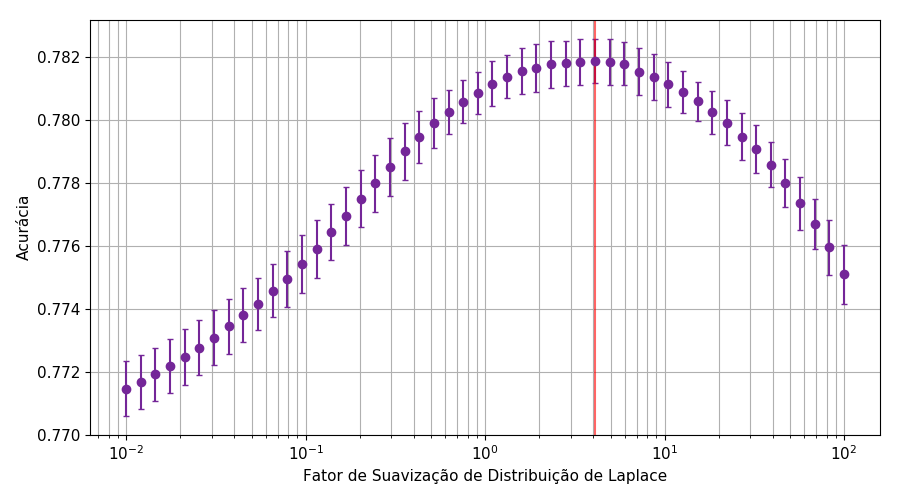
\includegraphics[scale=0.5]{go_nb.png}
    \caption{Seleção de hiperparâmetros de Naïve Bayes - Etapa 1.}
    \label{fig:go_nb}
    \end{center}
}
\end{center}
\end{figure}

A seleção do parâmetros do modelo formado por \textit{Support Vector Machines} foi feita por processo semelhante ao
anterior.
Foram variados o fator de regularização $L_{2}$, selecionando o modelo de maior acurácia média da validação cruzada.
A Figura~\ref{fig:go_svm} apresenta os resultados obtidos, no qual o fator de $6 \times 10^{-6}$ resultou na acurácia
média de 80.0\% sobre o conjunto de validação e 83,0\% de acurácia no conjunto de teste.

\begin{figure}
\begin{center} {
    \begin{center}
    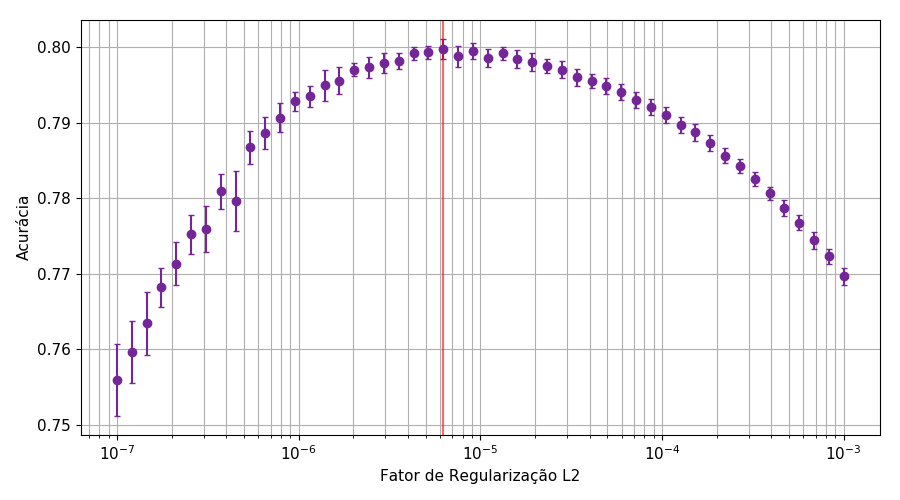
\includegraphics[scale=0.5]{go_svm.png}
    \caption{Seleção de hiperparâmetros de SVM - Etapa 1.}
    \label{fig:go_svm}
    \end{center}
}
\end{center}
\end{figure}

A Tabela~\ref{tab:go_compara} apresenta os resultados obtidos tanto no Sentiment140 quanto pela replicação de
seu método.
Pode se observar que foram atingidos valores próximos a referência, validando assim os pré-processamentos e as
implementações dos algoritmos aplicados.

% Resultados pós calibração
\begin{table}[h]
    \begin{center}
        \begin{tabular}{| l | r | r |}
        \hline
        \textbf{Algoritmo} & \textbf{Original} & \textbf{Replicação} \\ \hline
        Naïve Bayes & 81,3\% & 83,3\% \\ \hline
        SVM &  82,2\% & 83,0\% \\ \hline
        \end{tabular}
        \caption{Comparação de resultados da replicação dos classificadores do Sentiment140~\cite{go09}.}
        \label{tab:go_compara}
    \end{center}
\end{table}

\section{Segunda Etapa}

A segunda etapa consiste na validação do processo de formação de base de treinamento por supervisão distante.
A aplicação de técnicas de pré-processamento e algoritmos previamente validados neste novo conjunto de dados visa tanto
comparar o processo de elaboração por anotação ruidosa quanto servir como referência para a aplicação de algoritmos de
\textit{Deep Learning}.
Nesta etapa, os modelos serão avaliados tanto pelo seu desempenho na base de teste disponibilizada por Go
\textit{et al.} quanto aplicado na base de testes formada pela coletânea de \textit{tweets} oferecida pelas conferências
SemEval, como descrito na Seção~\ref{sec:data}

Assim como na fase anterior, foram treinados modelos por Naïve Bayes e \textit{Support Vector Machines}.
Neste caso, a seleção dos parâmetros de regularização foi feita de maneira a maximizar a área sob a curva ROC, visto que
os dados de treinamento apresentam desbalanceamento de classes.
As Figuras~\ref{fig:nb_selecao} e~\ref{fig:svm_selecao} mostram os resultados dos modelos, respectivamente, Naïve Bayes e
SVM a mudanças nos parâmetros de regularização, as linhas verticais vermelhas apontam os parâmetros que obtiveram maior
média de área sob a curva ROC dentre os grupos de validação quando aplicada validação cruzada com 10 partições.

\begin{figure}
\begin{center} {
    \begin{center}
    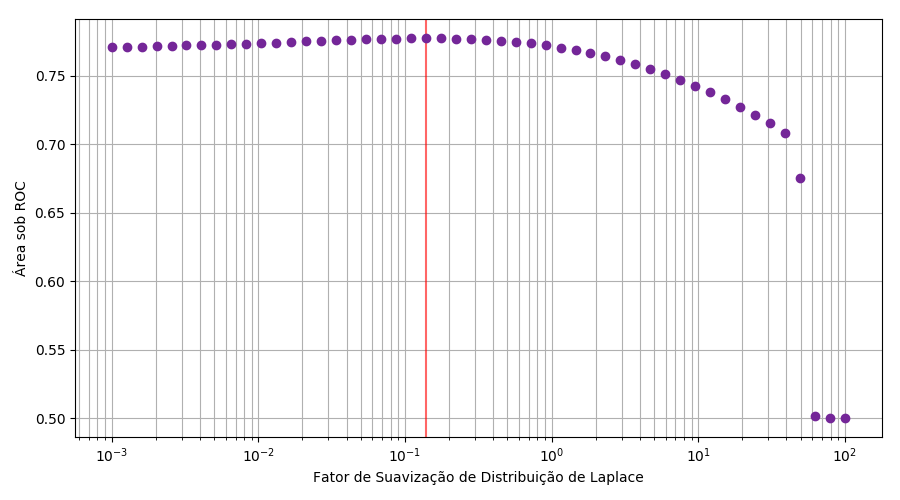
\includegraphics[scale=0.5]{nb_selecao.png}
    \caption{Seleção de hiperparâmetros de Naïve Bayes - Etapa 2.}
    \label{fig:nb_selecao}
    \end{center}
}
\end{center}
\end{figure}

\begin{figure}
\begin{center} {
    \begin{center}
    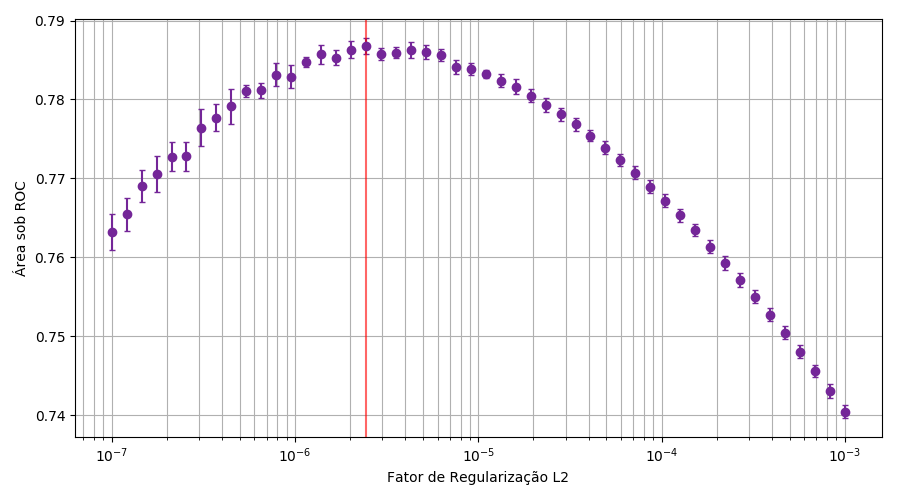
\includegraphics[scale=0.5]{svm_selecao.png}
    \caption{Seleção de hiperparâmetros de SVM - Etapa 2.}
    \label{fig:svm_selecao}
    \end{center}
}
\end{center}
\end{figure}

Uma vez selecionado os melhores hiperparâmetros, a Figura~\ref{fig:linear_roc_go} compara a curva ROC que caracteriza a
performance dos modelos treinandos tanto na primeira quanto na segunda etapa sob os dados de testes disponibilizados
por Go \textit{et al.}, a linha tracejada é utilizada como referência pois indica a performance de um classificador de
seleçao aleatória.
Observamos na Figura ~\ref{fig:linear_roc_go} que os modelos da etapa 1, treinados com os dados do Sentiment140,
obtiveram resultados semelhantes entre si e consideravelmente superiores aos classificadores da segunda etapa, treinados
com base coletada neste trabalho, dentre os modelos da segunda etapa SVM se sobressaiu em relaçao ao Naïve Bayes.

A Figura~\ref{fig:linear_roc_semeval}, por sua vez, apresenta a curva ROC dos modelos quando aplicados nos dados
manualmente anotados coletados do SemEval.
O compartamento dos classificadores nesta base de dados se assemelha ao observado anteriormente, porém, neste caso a
performance dos classificadores de SVM e Naïve Bayes da segunda etapa praticamente se igualaram.

\begin{figure}
\begin{center} {
    \begin{center}
    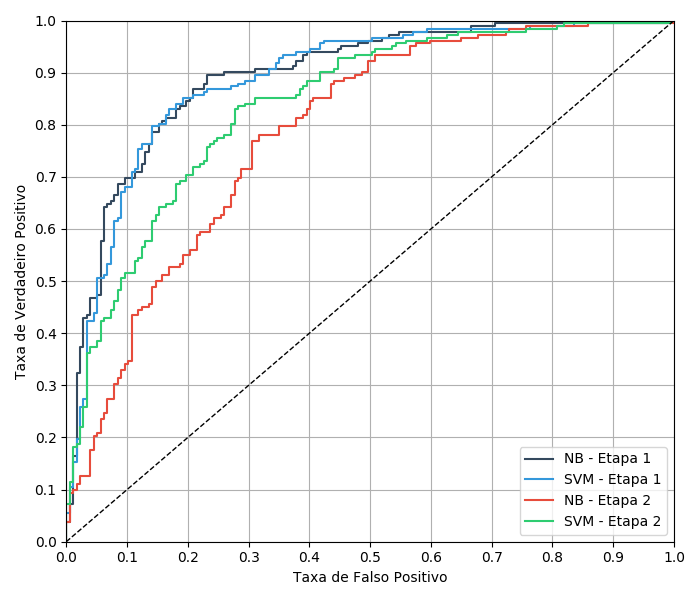
\includegraphics[scale=0.5]{linear_roc_go.png}
    \caption{Curva ROC dos modelos aplicados aos dados de teste do Sentiment140.}
    \label{fig:linear_roc_go}
    \end{center}
}
\end{center}
\end{figure}

\begin{figure}
\begin{center} {
    \begin{center}
    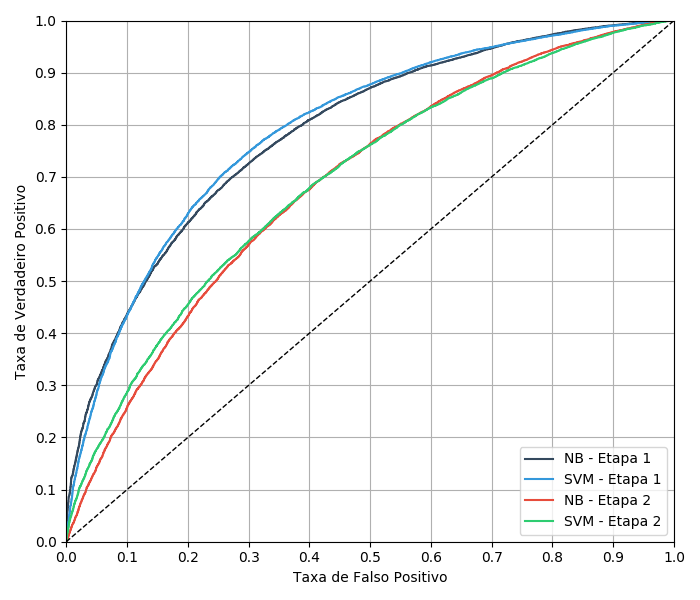
\includegraphics[scale=0.5]{linear_roc_semeval.png}
    \caption{Curva ROC dos modelos aplicados aos dados de teste do SemEval.}
    \label{fig:linear_roc_semeval}
    \end{center}
}
\end{center}
\end{figure}

Observa-se que os modelos treinados pelo conjunto de dados de anotação ruidosa disponibilizados por Go
\textit{et al.} apresentou desempenho consideravelmente melhor nos dois conjuntos de testes.
Desta maneira, se percebe que o processo de anotação dos dados foi mais ruidoso do que o apresentado pelo Sentiment140.

Uma hipótese a ser feita é que evoluções no idioma e na plataforma durante o intervalo entre a criação de ambas as
bases anotadas por supervisão distante tenha dificultado este processo, visto que a desenvolvida por Go \textit{et al.}
foi coletada em 2009, e a base de treinamento coletada por este trabalho conta com \textit{tweets} de 2017.
Constatou-se, por exemplo, que a base desenvolvida neste trabalho apresentou 1,1 milhões de palavras únicas após o
processo de tokenização, enquanto os dados de treinamento do Sentiment140 contam com 330 mil palavras únicas.

Outro fator relevante para definição de ruído no processo de anotação é a escolha dos \textit{emoticons}.
Neste trabalho, além dos \textit{emoticons} utilizados pelo Sentiment140, os \textit{emoticons} mais presentes nos dados
foram selecionados para classificação manual.
A escolha de \textit{emoticons} de maneira a atingir maior correlação com as classes pode ser uma solução para reduzir
a diferença de performance dos modelos entre os resultados de treinamento e os resultados de teste.

Apesar dos resultados obtidos na base de treinamento anotada para este trabalho serem inferiores aos apresentados pelos
classificadores treinados com a base disponibilizada por Go \textit{et al.}, a técnica de supervisão distante por
\textit{emoticons} para anotação ruidosa de mensagens de redes sociais se mantém como boa alternativa ao processo
custoso de anotação manual.

A Tabela~\ref{tab:linear_perf} resume os resultados dos modelos treinados na primeira e na segunda etapas quando
aplicados sob ambos os conjuntos de testes.
Ressalta-se nesta tabela que os resultados dos classificadores treinados na segunda etapa foram consideravelmente
inferiores aos da primeira fase e que os algoritmos de Naïve Bayes e SVM apresentaram ressultados semelhantes em
práticamente todas as situações, com excessão dos classificadores da segunda etapa aplicados na pequena base de teste
do Sentiment140.
O ponto de operação dos modelos foi escolhido de maneira a maximizar o índice SP.
É válido lembrar que a acurácia é uma métrica inconsistente quando consideras bases de testes com classes
desbalanceadas, como é o caso da base de \textit{tweets} coletados dos SemEval, sendo a área sob a curva ROC, AUC, ou o
índice SP, melhores opções para comparação destes casos.

% AUC -> CalibratedClassifier
% Acurácia, SP -> treshold: ponto de maior SP
\begin{table}[h]
    \begin{center}
        \begin{tabular}{ |l|l|l|r|r|r| }
            \hline
            \textbf{Dados de teste} & \multicolumn{2}{|c|}{\textbf{Modelo}}  & \textbf{Acurácia} & \textbf{AUC} & \textbf{SP} \\ \hline
            \multirow{4}{*}{Sentiment140} & \multirow{2}{*}{Etapa 1} & NB  & 83,3\% & 0,893 & 0,831 \\ \cline{3-6}
                                          &                          & SVM & 83,0\% & 0,887 & 0,830 \\ \cline{2-6}
                                          & \multirow{2}{*}{Etapa 2} & NB  & 73,3\% & 0,785 & 0,732 \\ \cline{3-6}
                                          &                          & SVM & 77,7\% & 0,839 & 0,776 \\ \hline
            \multirow{4}{*}{SemEval}      & \multirow{2}{*}{Etapa 1} & NB  & 70,9\% & 0,786 & 0,713 \\ \cline{3-6}
                                          &                          & SVM & 72,8\% & 0,791 & 0,724 \\ \cline{2-6}
                                          & \multirow{2}{*}{Etapa 2} & NB  & 64,9\% & 0,688 & 0,639 \\ \cline{3-6}
                                          &                          & SVM & 64,2\% & 0,693 & 0,640 \\ \hline
        \end{tabular}
        % FIX
        \caption{Resultados obtidos pelos classificadores.}
        \label{tab:linear_perf}
    \end{center}
\end{table}

\section{Terceira Etapa}

A terceira fase do projeto visa a reproduzir redes neurais convolucionais aplicadas a texto e comparar seu desempenho
a algoritmos de aprendizado de máquina consolidados no processamento de linguagem natural, como presentes na etapa
anterior.
Neste estágio, as redes serão treinadas com dados provindos da base anotada por supervisão distante, mesmos dados
utilizados para treinamento dos algoritmos de Naïve Bayes e \textit{Support Vector Machines} da segunda etapa.
Após feita a seleção dos hiperparâmetros, o modelo será avaliado aos treinados na segunda etapa com base no seu
desempenho obtido na base de testes disponibilizada pelas conferências SemEval.

Foram variados diversos hiperparâmetros, são eles: número de camadas, número de filtros convolucionais por camada,
tamanho dos filtros convolucionais, tamanho do filtro de \textit{pooling}.
Outros hiperparâmetros como: fator de regularização $L_{2}$ e probabilidade de Dropout foram mantidos fixos em
respectivamente $10^{-3}$ e $0,5$.
O valor escolhido de $\epsilon$, fator que define a estabilidade no treinamento, foi $10^{-3}$, o qual foi selecionado
após a análise de algumas curvas de treinamento.

A escolha dos hiperparâmetros foi feita de maneira a maximizar a área sob a curva ROC nos dados de validação.
A Tabela~\ref{tab:cnn_selection} lista os resultados obtidos por cada configuração treinada.

% apos treino coletar a auc de todos modelos (nos dados de treinamento mesmo), anotar valores na tabela
\begin{table}[h]
    \begin{center}
        \begin{tabular}{| >{\centering\arraybackslash}m{2.5cm} | >{\centering\arraybackslash}m{2.5cm} | >{\centering\arraybackslash}m{2.5cm} | >{\centering\arraybackslash}m{2.5cm}| c |}
        \hline
        \multicolumn{4}{|c|}{\textbf{Hiperparâmetros}} & \textbf{Resultado} \\ \hline
        \textbf{Número de Camadas} & \textbf{Número Filtros Conv.} & \textbf{Tamanho Filtros Conv.} & \textbf{Tamanho Filtros Pooling} & \textbf{AUC} \\ \hline
        \multirow{12}{*}{1} & \multirow{6}{*}{100} & \multirow{3}{*}{2} & 2 & 0.??? \\ \cline{4-5}
                            &                      &                    & 3 & 0.??? \\ \cline{4-5}
                            &                      &                    & 5 & 0.??? \\ \cline{3-5}

                            &                      & \multirow{3}{*}{3} & 2 & 0.??? \\ \cline{4-5}
                            &                      &                    & 3 & 0.??? \\ \cline{4-5}
                            &                      &                    & 5 & 0.??? \\ \cline{2-5}

                            & \multirow{6}{*}{200} & \multirow{3}{*}{2} & 2 & 0.??? \\ \cline{4-5}
                            &                      &                    & 3 & 0.??? \\ \cline{4-5}
                            &                      &                    & 5 & 0.??? \\ \cline{3-5}

                            &                      & \multirow{3}{*}{3} & 2 & 0.??? \\ \cline{4-5}
                            &                      &                    & 3 & 0.??? \\ \cline{4-5}
                            &                      &                    & 5 & 0.??? \\ \cline{1-5}

        \multirow{12}{*}{2} & \multirow{6}{*}{100} & \multirow{3}{*}{2} & 2 & 0.??? \\ \cline{4-5}
                            &                      &                    & 3 & 0.??? \\ \cline{4-5}
                            &                      &                    & 5 & 0.??? \\ \cline{3-5}

                            &                      & \multirow{3}{*}{3} & 2 & 0.??? \\ \cline{4-5}
                            &                      &                    & 3 & 0.??? \\ \cline{4-5}
                            &                      &                    & 5 & 0.??? \\ \cline{2-5}

                            & \multirow{6}{*}{200} & \multirow{3}{*}{2} & 2 & 0.??? \\ \cline{4-5}
                            &                      &                    & 3 & 0.??? \\ \cline{4-5}
                            &                      &                    & 5 & 0.??? \\ \cline{3-5}

                            &                      & \multirow{3}{*}{3} & 2 & 0.??? \\ \cline{4-5}
                            &                      &                    & 3 & 0.??? \\ \cline{4-5}
                            &                      &                    & 5 & 0.??? \\ \cline{1-5}

        \end{tabular}
    \caption{Seleção de hiperparâmetros de CNN.}
    \label{tab:cnn_selection}
    \end{center}
\end{table}

De acordo com a tabela, podemos observar que o conjunto de parâmetros com melhor desempenho no conjunto de validação
foram: X camadas compostas por Y filtros convolucionais de tamanho Z seguidas de \textit{pooling} com filtro de tamanho
W.
A Figura XYZ mostra a curva de treinamento deste modelo.

% TODO
FIGURA TREINO
% figura de treinamento com loss x val_loss, com legenda de cores e ressaltando a epoca selecionada

Uma vez selecionados os hiperparâmetros da rede neural convolucional, a Figura~\ref{fig:all_roc_semeval} apresenta a
curva ROC comparativa entre a rede e os modelos treinandos na segunda etapa quando aplicados a base de testes formada
por \textit{tweets} fornecido pelas conferências SemEval.
A Tabela~\ref{tab:all_compara} resume os resultados destes classificadores, novamente considerando que o limiar de
decisão foi selecionado de maneira a maximizar o índice SP.

% TODO - acertar figura
\begin{figure}
\begin{center} {
    \begin{center}
    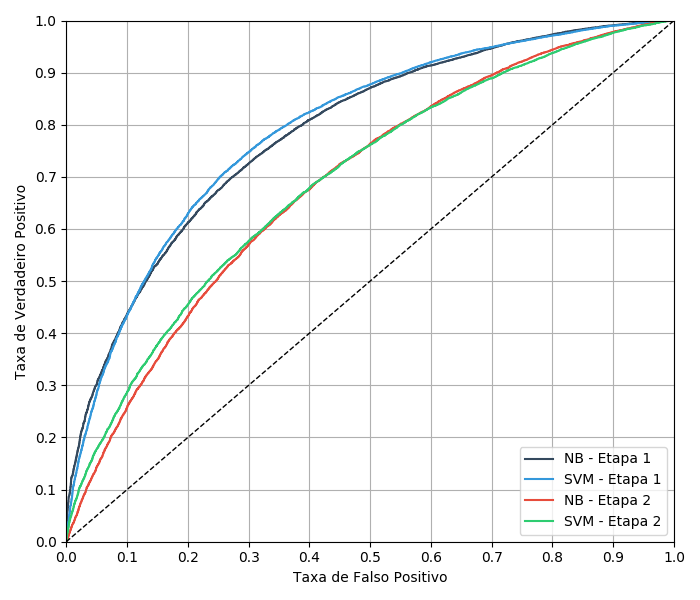
\includegraphics[scale=0.5]{linear_roc_semeval.png}
    \caption{Curva ROC comparativa dos modelos treinados por dados de supervisão distante.}
    \label{fig:all_roc_semeval}
    \end{center}
}
\end{center}
\end{figure}

\begin{table}[h]
    \begin{center}
        \begin{tabular}{| l | r | r |}
        \hline
        \textbf{Algoritmo} & \textbf{AUC} & \textbf{SP} \\ \hline
        Naïve Bayes & 0.688 & 0.639 \\ \hline
        SVM & 0.693 & 0.640 \\ \hline
        CNN & 0.??? & 0.??? \\ \hline
        \end{tabular}
        \caption{Comparação dos algoritmos treinados por dados de supervisão distante.}
        \label{tab:all_compara}
    \end{center}
\end{table}

Pode se observar que a utilização de redes neurais convolucionais em conjunto com representações obtidas por
\textit{embeddings} propiciou resultados melhores do que os obtidos com modelos tradicionais, como Naïve Bayes e
\textit{Support Vector Machines} sobre representações \textit{one-hot} dos textos.
Ressalta-se que a representação Word2Vec utilizada foi desenvolvida a partir de notícias.
O treinamento de modelos próprios para o meio no qual serão utilizados, neste caso, \textit{tweets}, pode melhorar o
desempenho do classificador a ser utilizado.


% ---------------------------------------------------------------
% Chapter 7 - Conclusões
% ---------------------------------------------------------------
\chapter{Conclusões}
\label{conclusao}
A massificação do uso das redes sociais gera uma crescente produção de dados.
Entretanto, as informações que estão sendo geradas são dispostas de forma não estruturada, dificultando sua extração.
Dado o volume de dados produzidos, torna-se cada vez mais custoso realizar esse processo manualmente.
Portanto, é fundamental o desenvolvimento de técnicas de processamento de linguagem natural capazes de auxiliar neste
procedimento.

O presente trabalho teve como objetivo o desenvolvimento de um método que gerasse classificadores de análise de sentimento
para redes sociais, sem uma dependência de anotação manual de bases de dados.
Classificadores formados por algoritmos de aprendizado de máquina vêm obtendo bons resultados na mineração de opinião.
Todavia, eles dependem de dados de treinamento, os quais têm produção custosa visto que sua criação depende da anotação
manual dos casos, dificultando, por exemplo, a reprodução destes classificadores para diferentes idiomas ou redes
sociais.

Para abordar este problema, foram estabelecidas três etapas.
A primeira etapa do desenvolvimento deste trabalho teve como objetivo replicar o artigo apresentado por Go
\textit{et al.}~\cite{go09} de maneira a validar os pré-processamentos e implementações de algoritmos observados.
Obtivemos acurácia de 83,3\% e 83,0\% pelos modelos utilizando Naïve Bayes e \textit{Support Vector Machine} respectivamente.
Estes valores estão próximos aos apresentados por Go \textit{et al.}, que obteve 81,3\% e 82,2\% com os modelos de Naïve
Bayes e SVM, nessa ordem.
Portanto, foi possível validar os pré-processamentos e a implementação dos algoritmos.

O segundo estágio deste projeto visou a avaliar a base de dados de anotação ruidosa formada para este trabalho
aplicando os mesmos modelos previamente validados.
Os resultados alcançados por modelos treinados nesta base de dados foram inferiores aos obtidos pelos modelos treinados
pela base de dados disponibilizada por Go \textit{et al.}
Concluímos que o processo de formação de base de dados por supervisão distante foi mais ruidoso do que o atingido por
Go \textit{et al.}
Entretanto, o método da anotação ruidosa por supervisão distante, apesar de apresentar dificuldades decorrentes da
seleção das características correlacionada com as classes, se mostrou eficiente na formação de bases de treinamento.

Os resultados obtidos na fase anterior serviram como base de comparação para terceira etapa.
Nessa etapa teve como finalidade analisar o desempenho de modelos de \textit{Deep Learning} aplicados a
análise de sentimento de \textit{tweets} e compará-los a algoritmos de aprendizado de maquina tradicionalmente aplicados
ao processamento de linguagem natural.
O modelo de rede neural convolucional alcançou o melhor valor de AUC, obtendo 0,738, superando Naïve Bayes e
\textit{Support Vector Machine} obtiveram 0,688 e 0,693 respectivamente.
Analisou-se então, que embora algoritmos de aprendizado de máquina tradicionalmente aplicadas ao processamento de linguagem
natural atinjam resultados positivos nesta tarefa, a utilização de técnicas de \textit{Deep Learning} é capaz elevar o
nível de desempenho obtido.
Observou-se também que é possível utilizar representações Word2Vec treinadas em notícias mesmo quando os objetos de análise
são mensagens de redes sociais.

Portanto, foi desenvolvido um método de produção de classificadores eficazes e que não dependem de anotação manual de
dados de treinamento.
Isso se fez possível pela utilização de representações de texto por algoritmos de aprendizado de máquina não
supervisionados e por classificadores compostos por redes neurais convolucionais, treinadas a partir de dados anotados
por supervisão distante.

\section{Trabalhos Futuros}

Uma das limitações da supervisão distante para a análise de sentimento é sua incapacidade de formar dados de treinamento
para classes neutras.
Aponta-se como um trabalhos futuros o desenvolvimento de técnicas de anotação ruidosa, ou novos métodos, capazes de lidar
com esse problema.

Outro fator a ser estudado é o desempenho na análise de sentimento de outros algoritmos da família de técnicas de
\textit{Deep Learning} que vêm obtendo sucesso em outras tarefas de processamento de linguagem natural e se mostram promissoras.
Um exemplo destas técnicas são as \textit{Long Short Term Memory}, esses modelos englobam em sua composição componentes
de memória temporal, que são fundamentais para análise de línguas.


% ---------------------------------------------------------------
% Bibliografia
% ---------------------------------------------------------------
\normalsize
\cleardoublepage
\addcontentsline{toc}{chapter}{Bibliografia}
\bibliographystyle{coppe}
\bibliography{biblio}

% ---------------------------------------------------------------
% Apêndices 
% ---------------------------------------------------------------
   \appendix
   % ---------------------------------------------------------------
   % Apêndice A
   % ---------------------------------------------------------------
   \chapter{O que é um apêndice}
   \label{ApendiceA}
   \paragraph{}Elemento que consiste em um texto ou documento elaborado pelo autor, com o intuito de complementar sua argumenta��o, sem preju�zo do trabalho. S�o identificados por letras mai�sculas consecutivas e pelos respectivos t�tulos.
   % ---------------------------------------------------------------
   % Apêndice B
   % ---------------------------------------------------------------
   \chapter{Encadernação do Projeto de Graduação}
   \label{ApendiceB}
   \begin{figure}
\begin{center}
\parbox[htb]{13.0cm}
  {
  \begin{center}
  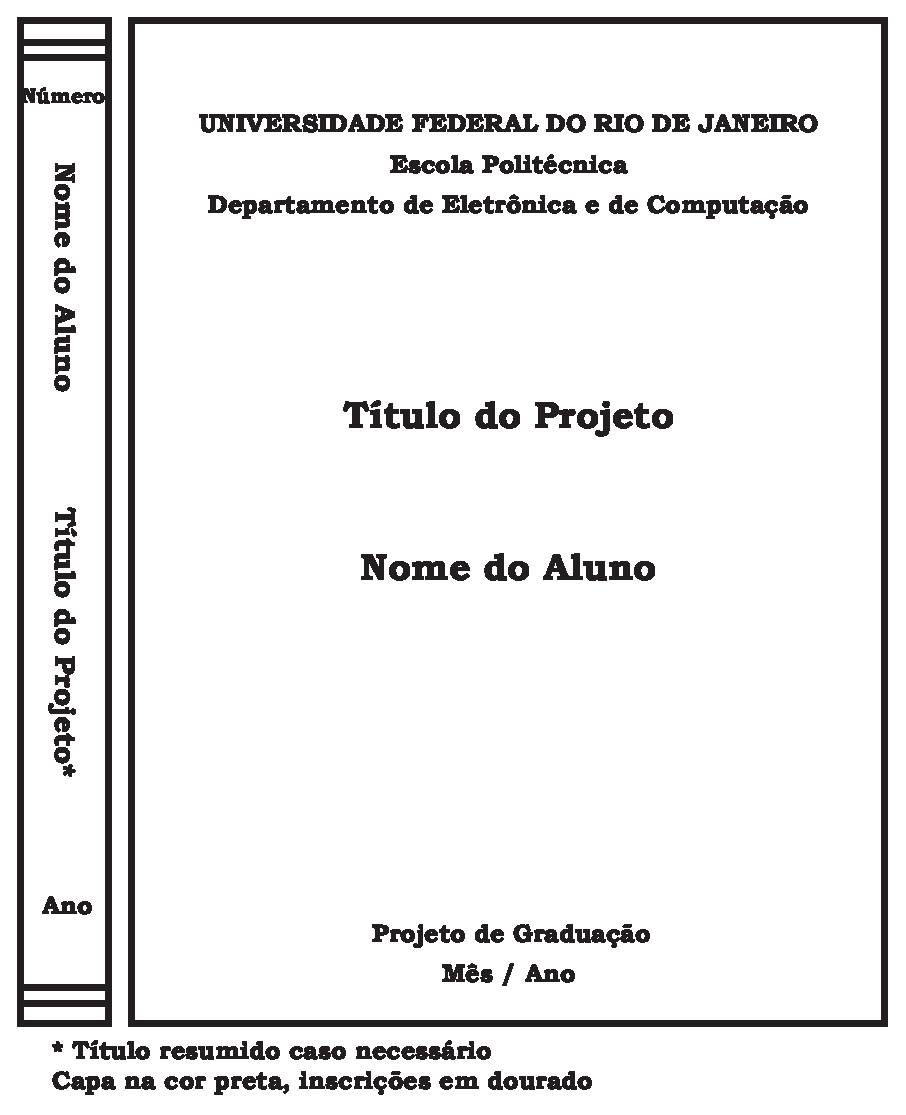
\includegraphics[scale=1.0]{Capa_do_Projeto_Final.eps}
  \caption[\small{Encaderna��o do projeto de gradua��o.}]{\label{FigPFC} \small{Encaderna��o do projeto de gradua��o.}}
  \end{center}
  }
\end{center}
\end{figure}
   % ---------------------------------------------------------------
   % Apêndice C
   % ---------------------------------------------------------------
   \chapter{O que é um anexo}
   \label{ApendiceC}
   \paragraph{}Documentação não elaborada pelo autor, ou elaborada pelo autor mas constituindo parte de outro projeto.   

\backmatter

\end{document}
